\documentclass[11pt]{report}
\usepackage{a4}
\usepackage{graphicx}
\usepackage{hyperref}
\usepackage{subfigure}

% For program-code:
\usepackage{listings}
\lstloadlanguages{C++,make}
\newcommand{\Cpp}{\lstset{language=C++,keywordstyle=\bfseries,breaklines,breakindent=30pt}}
\newcommand{\Make}{\lstset{language=make}}
\newcommand{\inl}[1]{\lstinline$#1$}

\Cpp

\begin{document}
\begin{titlepage}
\centering
\Large \textbf{The Core Language of C++11 by Examples}\\ \vspace{20pt}
Project Dissertation submitted to Swansea University\\ \vspace{6pt}
in Partial Fulfilment for the Degree of Master of Science in\\ \vspace{12pt}
\textbf{Advanced Computer Science with Specialization in Software Technology}\\ \vspace{30pt}
\large \textbf{Submitted by:}\\ \vspace{6pt}
\textbf{Dilshad H Sallo}\\ \vspace{6pt}
599502 \\ \vspace{30pt}
\textbf{Under the Supervision of:}\\ \vspace{6pt}
Dr. Oliver Kullman\\ \vspace{30pt}
\textbf{Project Conducted at:}\\ \vspace{6pt}
Department of Computer Science, Swansea University\\ \vspace{6pt}
Singleton Park, Swanse SA2 8PP, Wales, UK\\ \vspace{6pt}
September, 2012\\ \vspace{12pt}
\end{titlepage}



\begin{abstract}
C++11 is a new standard that released by C++ committee standard representing the effort of most experts in the world. This standard includes new features that addresses some limitations exist in traditional C++ as well as providing new features that never existed in any previous versions. These features are existed for supporting core language and some libraries as well as offering new facilities to make programming much easier and more functional.

The purpose of this project was to investigate core language and providing examples that represent cases of each feature to get most out of them, and demonstrating them as scientific catalogue to support programmers who have experience with programming in C++. Investigating core language was achieved by investigating; firstly, features that have significant impact to improve the runtime performance, secondly, features that primary existed to enhance usability of language for easier learning and understanding. Finally, features that improve functionality of language and offers something extraordinary that never existed.

This investigating is done by presenting features that belong to these three types with nice examples that give programmers clear idea about functionality of these features  and encourage them to shift toward C++11 style.

\end{abstract}

\begin{center}
\title \textbf{Acknowledgement}
\end{center}
\textrm{ First and foremost I want to gratefully and sincerely thank Almighty God for assisting me to complete this project. I owe special thanks to Dr. Oliver Kullmann for his excellent guidance, patience and most importantly, his friendship during doing this project.
\paragraph{} 
I would like to express special thanks to the Kurdistan Regional Government to fully support me during my study. I thank all my friends, my parents and all other family members for encouraging and supporting me throughout this study.
\paragraph{}
Finally, I give my deepest thanks to my wife Hanan for quiet patience and encouragement that make this work possible.}

\begin{flushright}
Dilshad H Sallo\\
599502\\
MSc Advanced Computer Science with specialisation in Software Technology\\
Swansea University\\
September 2012.
\end{flushright}

\tableofcontents
\listoffigures

\chapter{Introduction}
\label{cha:intro}
C++ is general-purpose programming language that is in widespread use for building small programs and substantial applications. C++ is designed to fully support three major concepts namely, object-oriented programming, data abstraction and generic programming which they have significant impact over evolution of programming. C++ has gained popularity and has become the choice of most programmers from around the world because it is extremely flexible, powerful and adaptable language. However, due to complexity of applications that required in a various fields and evolution of programming that accompanied by modern technology, some limitations and bugs have been discovered in C++ language that have significant impact on programmers of all backgrounds.  What is more, traditional C++ has lacking diverse functionalities which smoothly compatible with modern applications and has complicated syntax somehow that increases error-prone when attempting to write elegant and efficient code.  These deficiencies have negative influence over newcomers to language, and may encourage abandoning C++ towards other competition language. 

As responsibility of the ISO C++ standards committee to address these issues, new standard was released dubbed C++11, which is represented by new language features that have been added to core language, standard library and Standard Template Library. C++11 represents the effort of expert programmers who have Involved in C++ standard committee to develop the language abilities. C++11 has primarily existed to overcome some limitations that make traditional C++  undesirable in both educational and industrial fields, and also introduce new facilities to make programming more effective to its users. 

The aim  of this project is to investigate new language features that introduced by C++11 to core language and demonstrate them with suitable examples representing all cases of each features to be as scientific catalogue for supporting programmers who have sufficient programming knowledge in C++. These features are classified into three sections namely; runtime performance, usability enhancement and functionality improvement, and investigating core language properly require investigating into features that belong to these sections.

Features that belong to runtime performance section have primarily existed to increase performance of overall programs through, for example, avoiding duplicated copies that are take place when temporary objects are required to accomplish specific purpose.  Features that have introduced to usability enhancement section has substantial role of making language easier and safer to use by simplify the syntax and minimize code repetition through , for instance, using alternative mechanism that making code simpler and  much easier to learn and understand.  Finally, features that have added to functionality improvement section provide extraordinary capabilities that were previously impossible or extremely verbose such as allowing programmers to create their own literals which can be used to accomplish specific purpose. 

Core language features have been investigated and managed by using Git and Make tools which had significant role to achieve this project successfully. Git tool is used to keep tracking the modifications of programs that contributed in this project and manage them efficiently, while Make tool is used to compile and recompile the pieces of programs easily with helping file named Makefile, which contains all instruction that tell Make how to do work. 

This project gives unique opportunity for experienced C++ programmers for learning new style of programming as well as showing main usage for each feature in real examples. This will encourage C++ programmers to shift toward effective way of programming that make life easier.

\section{C++11}
\label{sec: C++11}
C++11 is the new standard of C++ language. It was known as C++0x until 2011, and then formally published as ISO/IEC 14882:2011(for main information see~\cite{Josuttis:2012:CppStandard},~p.~7) representative the effort of ISO C++ standards.  According to Bjarne (\cite{Stroustrup:2012:Cpp11}), "C++11 feels like a new language — the pieces just fit together better than they used to". C++11 provides new style of programming much more effective than before. C++11 is mainly existed to overcome the restriction and loopholes that make C++ inappropriate to build reliable and safe software.  C++11 introduces new facilities (features) which help programmers to think differently about system design and implementation (see~\cite{Stroustrup:2012:Cpp11}). This helping is not only restricted to C++ programmers but also for programmers who used to programming with other modern languages in general field. 

Features that introduced by C++11, extend the powerful of traditional C++ in terms of functionality, syntax and efficiency as well as enabling programmers to write robust code in high-level style. Moreover, the improvement of general abstraction mechanisms are also supported (for more information see~\cite{Stroustrup:2012:Cpp11}) and can be more flexible and safe by combining some features together. C++11 able to cover some limitations that existed in C++ and reduces the overall verbosity through providing new concepts such as lambda expressions and auto keyword, which increase its overall expressiveness, clarity and  reduce amount of codes and make C++ more usable language.

C++11 adds some significant features such as rvalue references and move semantic (for more details see~\cite{Gregorie:professionalcpp},~p.~278) that improves the basic efficiency of the language and allow developers to implement faster code. Last but not least, C++11 bring new features to standard library which never existed in any previous versions and they have significant impact to support generic programming (see~\cite{Stroustrup:2012:Cpp11}), including multi-threading support directly into C++ and smart pointers that will simplify memory management.

\section{Why C++11?}
\label{sec: why C++11}
According to Bjarne (\cite{Stroustrup:2005:Cpp}), the nature of C++ focuses on supporting general features (especially classes) to demonstrate its primary strength, whereas it has main weakness that represents the deficiency of specialized features (such as thread). C++11 is not  only  support specialized features, contrariwise it offers new features that reinforce both sides simultaneously, because C++ is a general purpose language and is not just designed to build "windows applications" or "web languages". C++11 will be compatible with C++, and will provide new features that are neglected clearly by existing Standard C++. This includes supporting for distributed and parallel programming, a concurrency which gains obvious popularity these days.

C++ is almost becoming favourite language for expert programmers to build sophisticated software that are required by modern technology. However, it do not provide enough supportive libraries that assist novice programmers because language itself not able to support everything. C++11 provide diversity of separate libraries that have significant impact to support programmers of all backgrounds (for addition information see~\cite{Stroustrup:2005:Design}). Furthermore, standard library and language (core language) are also extended to contain various features that make programming much easier to understand and with less error-prone.

The key to robust and sophisticated code is type safety using an appropriate type system, which ensures that errors are not propagated within programs. C++ does not consider completely a type safe system, because many implicit conversions and narrowing conversions could happen during some operations that lead to incorrect behaviour of programs. C++11 cannot make C++ entirely type safe, but it will not bring new loopholes that make system unsafe (for main information see~\cite{Stroustrup:2005:Cpp}). In addition, it introduces new facilities that used to inhibit ambiguity behaviour by alternative mechanism to current insecure practices.


\section{What has been achieved}
\label{what has been achieved}


\section{Why small and many programs?}
\label{sec:small and many programs}
knowing the syntax of C++11 language is not enough to learn and understand the correct way to use the language efficiently, unless providing  simple  programs that give idea to programmers from first glance. These programs represent features of core language and their cases which could differ from usage to other. As C++11 provides capabilities and new style of programming, it become much easier to represent each feature in real example and give elementary idea to programmers to become able to build complex software as final target.

% Boost 
\section{Boost C++ libraries}
\label{sec: Boost}
The Boost C++ libraries "are free, open-source libraries" (see~\cite{Deitel:2012:CPP},~p.~31) created by the very same developers who designed and build the C++ standard libraries. They are designed to extend the functionality of C++ language in an efficient and commercial-grade, universally applicable style. Boost C++ libraries introduces helpful and well-designed libraries that regard compatible with C++ Standard Library (for more information see~\cite{Deitel:2012:CPP},~p.~937) and majority of which have been accepted in the C++ Standards Committee's Library Technical Report (TR1). In addition, parts of Boost library are currently being accepted into the Standard library for C++11 (see~\cite{Boost:2007:Cpp}) and they are regarded as one of the top libraries with a high industry acceptance. These libraries are Boost.Array, Boost.Bind, Boost.Function, Boost.Random, Boost.Regex, Boost.Smart\_ptr, Boost.Tuple and Boost.Type\_traits.

As a result, the current C++11 Standard libraries include several more Boost libraries in addition to those from TR1 and they provide many features that making Standard Library powerful and more effective in both industrial and educational fields.

\section{A brief history of C++}
\label{sec: History of C++}
The history of C++ programming language has begun in 1979, when Bjarne Stroustrup was working on his Ph.D thesis in the Computing Laboratory of Cambridge, University of England (see~\cite{StroustrupHistory}). At that time, he had opportunity to work with a language called Simula (for more information see~\cite{Stroustrup:2012:Cpp11}), which was considered as the first language that supports the object-oriented language paradigm. He observed that Simula had very useful features for developing great software, but it was extremely slow in terms of practicality.Shortly thereafter, Bjarne Stroustrup commenced working on a new language dubbed "C with Classes" (see~\cite{StroustrupHistory} for addition information), which represented improvement version of C language. This enhancement was done by adding a number of new features that borrowed from the esoteric language Simula. The most notable of which were classes that have capability for supporting object-oriented programming . 

During 1982, Bjarne Stroustrup found that "C with Classes" was not quite enough successful to become useful and attractive language that paid to develop organization (see~\cite{StroustrupHistory}). Bjarne had only two options that must be taken regarding to "C with Classes" (for more details see~\cite{Stroustrup:1994:DesignEvolution},~p.~63) either cease supporting this language, or use his experience with "C with Classes" to develop new language that able to develop and support lager organization.

In 1983, the name of the language was changed from "C with Classes" to C++. According to Bjarne (\cite{Stroustrup:1994:DesignEvolution},~p.~64) the name of C++ was picked because it was short and had precise interpretations. In C, "++" operator is the C increment operator, indicating evolution from changes of C.  Around this time, a lot additional features were added to the language and the most known of which are references, constants~(const), functions overloading and virtual functions.

In 1985, Stroustrup's reference to the language titled The C++ Programming Language was published. C++ was carried out as a commercial product in the same year though it was not officially standardized. The language was updated again in 1989 (see~\cite{CplusplusHistoryofCpp}) to include protected and static members, as well as multiple.

In 1990, the Annotated C++ Reference Manual was released, which became as basis for the future standard. At that time, many significant features were added to C++  (for main information see~\cite{StroustrupHistory}) included namespaces, new casts, exceptions, Boolean type and template.

In 1998, the standardization of C++ published the first international standard for C++ under official title; Information Technology -- Programming Languages -- C++ (for main information see~\cite{Josuttis:2012:CppStandard},~p.~7). This standard would be known as C++98 and has document number is ISO/IEC 14882:1998. The Annotated C++ Reference Manual has an important influence on the development of the standard (see~\cite{CplusplusHistoryofCpp}). In addition it was included the Standard Template Library which started its conceptual development in 1979. Due to multiple problems and bugs have discovered in C++98, the standardization of C++ revised it accordingly, and release revision standard in 2003 to ensure greater portability and consistency dubbed C++03 (for main information see~\cite{Josuttis:2012:CppStandard},~p.~7), which has document number ISO/IEC 14882:2003.

In 2005, the standardization of C++ issued a Technical Report 1 that contains library extensions for the latest C++ standard (see~\cite{Josuttis:2012:CppStandard},~p.~7). The proposed changes for new standard was informally dubbed C++0x (see~\cite{CplusplusHistoryofCpp}), which considered as working name for the next standard of C++. Its first draft for formal comments was produced in September 2008. 

In 2011, C++0x was officially approved as C++11 and published as the second standard. This standard has officially entitled as "Information Technology — Programming Languages — C++" and its document number is ISO/IEC 14882:2011 (for further information see~\cite{Josuttis:2012:CppStandard},~p.~7). According to Bjarne (\cite{Stroustrup:2012:Cpp11}), the 11 in the name of new standards refers to the year of publication that release in. C++11 came with new features that have substantial improvement over the core language and library. C++11 provided new facilities that make life easier for programmers of all backgrounds as well as introducing new programming style  that make the language more easier to learn and understand.

% overview
\section{Overview}
\label{sec:Overview}
The list below show the organization of the chapters which constitute this dissertation.

\textbf{Chapter~\ref{chapter: Runtime Performance Enhancements}} covers investigation of  features that provide some kind of benefit to runtime performance. Improve the performance of overall programs  can be achieved, for example, by applying the concept of move semantic that able to move temporary objects instead of creating deep copies of them. More  features that have important impact over runtime performance can be found in this chapter. \textbf{Chapter~\ref{chapter: Usability Enhancements}} looks into features  that enhance the language through simplify the syntax  and make it more usable. This can be done for instance through using auto keyword that able to deduce the data type from initialization and reducing the complexity of code. This chapter includes many features that make programming much more easier to write,learn and understand. \textbf{Chapter~\ref{chapter: Functionality Improvements}} deals with investigation of features that improve the functionality of language and offers something extraordinary. This chapter includes some features that extend functionality of several previous features in traditional C++  such as long long int that extend long int to guarantee more usable bits, others provide something that never existed for example user-defined literals which give a user the ability to create new custom literal modifiers. \textbf{Chapter~\ref{cha: tools}} describes how Git and Make tools have used to develop this project successfully by recording the changes that happen during development and compiling and recompiling source files to build executable files by typing make. More details about these significant tools can be found in this chapter. \textbf{Chapter~\ref{chapter: conclusion}} provides a summary of the dissertation, and considers possible future work that could be done to fully extend this project  as well as showing my personal project experience.


% chapter Core Language Runtime Performance Enhancements
\chapter{Core Language Runtime Performance Enhancements}
\label{chapter: Runtime Performance Enhancements}
C++ is one of the most powerful programming languages that use to create reliable and robust large scale applications (for overview of C++ see~\cite{Stroustrup:2012:Cpp11}). It is widely used in application that requires high performance due to its nature to create software that is efficient in time and space. However, there are some aspects which have substantial effect every time a program is run and leading to slow the performance of entire program.  These could happen when needing to create deep copy of temporary object that use to copy from source object to target object. Thus, two exactly copies of object are existed at a runtime. Another reason is that, all initialization of objects and built-in types are took place at runtime, and if any computation is happened during compile-time, it is also repeated at run time and leading to slow performance of program and make it costly. To overcome these issues, C++11 introduces several features that have significant impact over runtime performance and they provide control to a programmer to increase a runtime performance.

In this chapter we explain how C++11 able to increase the performance of overall programs by providing some important features such as rvalue and move semantic which used to prevent deep copies by moving temporary objects instead of creating them; generalized constant expressions which ensure that when some computation or initialization of object and fundamental types are happened at compile time and will not repeat at runtime, and new style of POD for allocating memory from free store without runtime overhead.

The topics of this chapter include rvalue references, move semantic, generalized constant expressions and Modification of the definition of plain old data.


\section{Rvalue references}
\label{section: Rvalue references}
A reference in C++ is an alias or alternative name for an existing object, and any modification could be done through this reference, will affect the original (for addition information see~\cite{Gregorie:professionalcpp},~p.~286). Traditional C++ supports lvalue references, which are used to reference to lvalues. Lvalues can be represented by single variable or persistent object that located on the left-hand side of an assignment operator. All variables, including~(const) variables are Ivalue. On the other hand, rvalue defined as anything is not lvalue, such as temporary object and constant value that appeared on the right- hand side of an assignment operator (for further information see~\cite{Gregorie:professionalcpp},~p.~277). Lvalues can be used as rvalues, but not vice versa. In traditional C++, non-const references can bind to lvalues, and const references can bind to either lvalues or rvalues. However, there is nothing that can bind to a non-const rvalue (see~\cite{Stroustrup:2012:Cpp11} for more details). Therefore, a reference to a temporary and a constant are not supported in traditional C++.

C++11 brings new concept called an rvalue reference, which bind only to rvalues but not to lvalues. Rvalue references use two ampersands (\&\&) rather than one (\&), and can be const and non-const (see~\ref{RvalueReference_Basic}), the same as lvalue references  (for main information see~\cite{Gregorie:professionalcpp},~p.~277). Rvalue references can be used as a parameter to function by using two ampersands as part of the parameter specification such as type \&\& name. Then, this function can be only invoked when a parameter is a temporary object or constant value (more information can be found in~\cite{Gregorie:professionalcpp},~p.~277). Otherwise, function that takes lvalue references will be invoked by lvalue (see~\ref{RvalueReference_Parameter}). However, while rvalue reference will never be bound to an lvalue, it is possible by a programmer to force a compiler to convert an lvalue into an rvalue (see~\cite{Gregorie:professionalcpp},~p.~278). This can be done by using new feature called \texttt{std::move()}, which added by C++11 (see~\ref{RvalueReference_Move}).

Rvalue references can also be used as a parameter to a function template but with nuance in terms of implementation. Calling the function with rvalue, leading the type parameter is deduced to be value. However, if an lvalue is passed to the function, then the type parameter is deduced to be an lvalue reference (for more details see~\cite{Williams:2012:CCA},~p.~318). Due to the function parameter is declared as rvalue reference (type \&\& name), that is, it treats as a reference to a reference for original reference type. Thus, a single function is able to accept both rvalue and lvalue parameters (see~\ref{RvalueReference_Template}). This is pretty useful to execute perfect forwarding, which means that a function template able to pass its arguments by to another functions while keeping the rvalue and lvalue nature of the function arguments (see\cite{Williams:2012:CCA},~p.~319 for more information). This avoids excessive copying and avoids the template author having to write multiple overloads for rvalue and lvalue references. Therefore, this concept is essential for library features such as \texttt{std::thread} and \texttt{std::function} which pass arguments to another function (see~\ref{RvalueReference_Forwarding}).

One of the main reasons for introducing the rvalue reference is to implement move semantics, the next topic in this chapter.

% Move semantic
\section{Move semantic}
\label{section: Move semantic}
C++ is always used to create fast and robust programs that be trusted in different areas. However, one of the cases that lead to slow down the performance of many C++ programs is the creation of temporary objects. Usually, these temporary objects are created by copy constructor and assignment operator because they need a second object (temporary object) that should be equal to the original to accomplish operation (for addition information see~\cite{Stroustrup:2012:Cpp11}); therefore, once the operation is done a program has two objects with the same value that resulting in expensive object copies.

C++11 introduces the concept of move semantic, which allows an object to be implemented by a move constructor and a move assignment operator (see~\cite{Gregorie:professionalcpp},~p.~278). These concepts are used by a compiler when the second object is temporary object and is going to be destroyed after the copy or assignment. Both the move constructor and the move assignment operator transfers resources such as variables and pointers from the source object that is temporary object, to the new object (target object) and then reset the variables and pointers of the source object to null values. This would be similar to moving a file from one directory to another. By doing this, the ownership of the memory will be move from the source object (temporary object) to the new object (target object). In fact, move constructor and move assignment operator do a shallow copy of the resources and switch ownership of allocated memory (for more details see~\cite{Gregorie:professionalcpp},~p.~280) to prevent memory leaks or dangling pointers. Thus, move semantic is a significant concept to increase the performance of programs by avoiding unnecessary copies that used in temporary objects.

The implementation of move semantics is supported by rvalue references, which should be added to class to implement move constructor and move assignment operator. Move constructor is pretty useful, and its purpose is to steal as many resources as it can from the original object, as fast as possible, because the original does not need to have a meaningful value any more. Thus, it is going to be destroyed. Move constructor can be tested with class C that contains copy constructor and move constructor as follows:

\begin{lstlisting}
class C {
public:
  C(int);
  C(C&& c);
  // Remaining code omitted for brevity
}
\end{lstlisting}
When move constructor exists, it will be used by a compiler to move the temporary objects instead of copy them and without needing for any deep copy. The implementation of move constructor and move assignment are as follows:
\begin{lstlisting}
C::C(int i) : n(i), p(new int[i]) {
  std::cout << "Normal Constructor." << std::endl;
}
C::C(C&& c) : n(c.n), p(c.p)  {
  std::cout << "Move constructor." <<std::endl;

  //Reset the source object
  c.n = 0;
  c.p = nullptr;
}
\end{lstlisting}

The move constructor will be invoked by a vector to move old vector to the new one and bigger vector as follows:
\begin{lstlisting}
int main() {
  std::vector<C> v;
  v.push_back(C(10));
  v.push_back(C(20));
}
\end{lstlisting}

Therefore, the output of class C will be as follows:
\begin{enumerate}
\item Constructor called.
\item Move constructor called.
\item Constructor called.
\item Move constructor called.
\item Move constructor called.
\end{enumerate}

In the beginning, the vector is created and still empty, until first line of code will be executed:
\begin{lstlisting}
v.push_back(C(10));
\end{lstlisting}

Then, a new C object is created by invoking the normal constructor~(1); after that, a vector will resize itself to accommodate a new object, which is going to push in. The C object that created will move into the vector by calling the move constructor~(2). When the second line of code is executed:
\begin{lstlisting}
v.push_back(C(20));
\end{lstlisting}

A second C object is also created by calling the normal constructor~(3). At this point, the vector can store one element, so once again it is resized to accommodate a second object. When the resizing is done by the vector, the objects that previously have added require to be moved from the old vector to the new and larger vector, so this will require invoking the move constructor for objects that previously have added~(4). And then, the new C object is moved into the vector by invoke move constructor~(5) (see~\ref{MoveSemantic_Constructor} for complete example)(for main information see~\cite{Gregorie:professionalcpp},~p.~281). As a result, the move semantics is efficiently performed the insertion operation for vector by moving the elements rather than copying them.

The move assignment operator can also be tested by another class C which contains copy assignment and move assignment as follows:
\begin{lstlisting}
class C {
public:
  C& operator=(const C&) { 
  std::cout << "Copy assignment Operator." << std::endl; return *this; 
}
 C& operator=(C&& c) {
  std::cout << "Move assignment operator." << std::endl;
  if(this == &c) {    //check for self-assignment
    return *this;
  } else {
   delete [] p; // Free the existing resource.

  i = c.i;    // shallow copy of data
  p = c.p;    // shallow copy of data

  c.i = 0;  //Reset the source object
  c.p = 0;  //Reset the source object
  }
  
  return *this; 
}
C createObject() {
  return C(1);
}
 // Remaining code omitted for brevity
}
\end{lstlisting}

Class C has function called createObject() that create temporary C object ("as a return type is always rvalue") and assign it to another object called c1 as follows:
\begin{lstlisting}
c1 = createObject();
\end{lstlisting}

Resulting to invoke the move assignment operator (for more details see \cite{Gregorie:professionalcpp},~p.~282). The move assignment operator is also invoked by using \texttt{std::move()} ("which converts from lvalue to rvalue") to assign one object that consider temporary object to a target object, as follow:
\begin{lstlisting}
c2 = (std::move(c1)); // call move assignment operator
\end{lstlisting}

On the other hand, the assignment \texttt{(c3 = c1)} will invoke the copy assignment operator because the object c1 is not temporary object, but a named object (see~\ref{MoveSemantic_AssignmentOperator} for complete example).

Another situation that uses move semantic to increase the performance, when swap of elements are required. This can be done by using \texttt{std::move()}, which is the C++11 way to use move semantics explicitly and can be used to transfer the content of an object somewhere else, without doing a copy (for addition information see~\cite{Gregorie:professionalcpp},~p.~282). This will lead to raise the performance of programs that require a lot of swaps (see~\ref{MoveSemantic_Swap}).

% Generalized constant expressions
\section{Generalized constant expressions}
\label{section: Generalized constant expressions}
C++ had the notion of constant expressions such as 1+2, that always yield the same results at compile-time and at run-time. Such these expressions are improvement opportunities for a compiler to execute them at compile-time and gain the results in a program rapidly. Constant expressions required in some circumstance that should meet C++ specification, including enumeration values and specifying the bounds of an array. Currently, they can be expressed in C++ by using the keyword const, which could appear with variables, indicating that cannot be altered.

However, the C++ rules concerning constant expressions are overly restrictive. They obligate some usage such as macros or template meta-programming instead of inline functions to guarantee the compile-time evaluation of constant expressions (for more details see~\cite{Stroustrup:2012:Cpp11}). This could happen for example when using class template \texttt{std::numeric\_limit<>::max}. Seemingly, they should be used as an integral constant but in fact it is functionally equivalent to the macro INT\_MAX. Thus, they are not integral constant. Therefore, this encourages users to favour macros when values require to be known at compile time. Another restriction could be found in C++, when return type of function is used for specifying the bounds of an array (for further information see~\cite{Stroustrup:2012:Cpp11}). This causes compilation error because a compiler has no way of knowing the return function will be constant at runtime.

Due to these restriction, C++11 has extended the constant expressions by introducing the "constexpr" keyword that dubbed generalized constant expression. The constexpr keyword allows certain computations happen at compile-time instead of run-time when the program itself is run (for addition information see~\cite{Williams:2012:CCA},~p.~324). This has apparent benefit in terms of performance, due to anything could be done at a compiler-time, will be done once, and instead of every time the program runs. Hence, a program takes the advantage of compile-time, and leading to increase performance of a program.

\subsection{Constant-expression data}
\label{subsection: constant-expression data}
The constexpr keyword can be applied to variables and data members. Variables or data members that are declared with this keyword are named a constant-expression value, and they only allowed initializing with constant expressions (for main information see~\cite{Williams:2012:CCA},~p.~324). Variables and data members that declared with constexpr keyword have the same behaviour as if they were declared const. However, there is one difference namely, they need initialization before they are used and should be a constant-expression to guarantee that constexpr variables and data members can always be used as a constant expression (see~\ref{Constexpr_Data}). 

\subsection{Constant-expression functions}
\label{Constant Expression Functions}
A constant expression function is a function that can be performed at compile time by means of inlining and assessing the result at compile-time. Declaring a function as constexpr enforces a few requirements that must be followed regarding as a constant-expression function (see~\cite{Gregorie:professionalcpp},~p.~287 for further information); otherwise, declaring it constexpr is a compilation error. The requirement necessary for a constexpr function are as follows:

\begin{enumerate}
\item The body of function must consist of single return statement and must be in form {return expression ;} where expression must evaluate to a constant expression after substitution.

\item Any parameters to the function must be a literal type or reference to literal type.

\item The return type of function must be a literal type. It cannot be void.

\item Function can call only other constexpr functions (see~\ref{Constexpr_Recursion}).

\item If the constexpr function is defined as member of a class, the function cannot be virtual.
\end{enumerate}

Applying these requirement enable a compiler to evaluate a constexpr function at compile time. Thus, it becomes possible as follows to use the return type of constexpr function to specifying the size of an array (see~\ref{Constexpr_ArraySize} for complete example).
\begin{lstlisting}
constexpr int getsize (int i) { return i * i;}
int main() {
  int array[getsize(3) + 6] = {0};
  // Remaining code omitted for brevity
}
\end{lstlisting}

However, recursion in this type of function is not restricted and can be applied ("evaluate at compile-time") by using the ternary operator (? :)(for main information see~\cite{Allain:2011:FutureCpp}) as a single return statement as follows:
\begin{lstlisting}
constexpr int fact (int n) {
  return n > 0 ? n * fact( n - 1 ) : 1; // recursion function
}
\end{lstlisting}

Hence, a compiler can optimize away the call and make the computation all at runtime. In this case, by permitting more complex computation, constexpr acts differently than a just in-line function, because an in-line recursive function is not possible, lead to consider function argument is itself a constexpr and be computed at compile time (see~\ref{Constexpr_Recursion} for complete example). Last but not least, constexpr function can also be involved at runtime (for further information see~\cite{Allain:2011:FutureCpp}). This can be done when the arguments to the function are declared as non-constant. Therefore, there is not required for creating separate functions to be executed at compile time and run time as long as it offers a convenient way to define function that work at compile time as well as runtime (see~\ref{Constexpr_FunctionRuntime}).

\subsection{Constant-expression constructors}
\label{subsection: Constant Expression Constructors}
A constant expression constructor allows creating user-defined types (such class) as constant expression (\cite{Gregorie:professionalcpp},~p.~287). This can be done by defining a constructor with constexpr keyword as follows:
\begin{lstlisting}
class Rectangle {
public:
  constexpr Rectangle(int i, int j) : width(i), height(j) {}
  constexpr int get_width() { return width;}
  constexpr int get_height() { return height;}
  // Remaining code omitted for brevity
}
\end{lstlisting}
 Defining constexpr constructor must also meet following criteria:
 
\begin{enumerate}
\item	The body of constructor must be empty.
\item	All arguments of constructor must be literal types or references to literal types.
\item   All non-static data member must be initialized.
\item	The body of constructor cannot be a function-try-block.
\item	All data members must be initialized with constant expressions.
\end{enumerate}
The constant expression evaluation happens in the member initializations which must fit the requirement ("arguments must be constants") to evaluate as constants. An object that construct with a constant-expression constructor and constant expression arguments, is named as user-defined literal and can be used at compile time to specify the bound of array via its methods as follows:
\begin{lstlisting}
constexpr Rectangle rect(2,3);
constexpr int multidimensional[rect.get_width()][rect.get_height()] = {{0}};
\end{lstlisting}
For complete example about constant expression constructors (see~\ref{Constexpr_ConstantConstructor}).

% modification of the definition of POD
\section{Modification of the definition of plain old data}
\label{section: Modification of the definition of plain old data}
Plain old data~(POD) is a data structure that represented with fundamental types, without using the object oriented features, to suggest areas of essential compatibility between comparable data types in C and C++ (for addition information see~\cite{Stroustrup:2012:Cpp11}). A POD type in C++ is classified as either a scalar type or a POD class. The scalar type collectively refers to the fundamental types of C++ such integral types (int, char), floating types (float, double), enumeration types and pointer types. Whereas the POD class has no non-static data (including arrays) of any pointer-to-member type, no non-static data~(including arrays) of any non-POD class type, no user-defined copy assignment operator, nor user-defined destructor (see~\cite{MSDN:2012:CppModern} for more details). In addition, a POD class has to be an aggregate, meaning it has no private or protected not static data members, no user-declared constructors, no base classes and no virtual functions.

In the traditional C++, the actual definition of POD is based on a set of restrictions that should be satisfied for defining POD class or structure; otherwise, it is not POD type. Therefore, C++ able to distinguish between POD types and non-POD types. However, in some situations, this distinction is limited, because some non-POD types have similar properties as POD types. Thus, they have the same behaviour.

C++11 relaxed some of the POD rules by dividing the POD concept into new type categories: trivial classes and standard layout classes and their definition no longer depends on the definition of aggregate (for more information see~\cite{MSDN:2012:CppModern}). A trivial class can be statically initialized and can be copied via \texttt{memcpy()}, instead of having to use a copy constructor. The lifetime of a trivial type begins when its storage is defined, not when a constructor completes. The trivial class is a class that:
\begin{enumerate}
\item	Has a trivial default constructor. 
\item	Has a trivial copy and move constructor.
\item	Has a trivial copy and move assignment operator.
\item	Has a trivial destructor.
\end{enumerate}

Additionally, trivial class has no virtual member functions of the class and no virtual base classes (see \cite{ISO:2011:Cpplanguage},~p.~215 for further information). Hence, it can have user-defined constructors as long as above requirements are available (see~\ref{POD_TrivialClass}).

Standard layout is intended to capture the first intent by creating something with a layout the same as getting in C. A standard layout class is a class (for more information\cite{ISO:2011:Cpplanguage},~p.~216) that has follows requirements:

\begin{enumerate}
\item	Has no virtual functions and no virtual base classes.
\item	Has no non-static data members of type non-standard-layout class (or array of such types) or reference.
\item	All its non-static data members have the same access control (public, private, protected).
\item	It has no base classes of the same type as the first defined non-static data member (see~\ref{POD_StandardLayoutClass}).
\end{enumerate}

A class or structure is considered POD type if it is trivial, standard-layout, and all of its non-static data members and base classes are PODs (see~\ref{POD_StandardLayoutandTrivialClass}). By separating trivial and standard-layout concepts, it becomes possible to give up one without omitting other (see~\cite{Stroustrup:2012:Cpp11} for more details). A class that has copy  and move constructors could not be trivial, but it may be may be standard-layout and hence interrupt with C. Likewise, a class that has  public and private non-static data members may not be standard-layout, but it could be trivial and hence, can be copied via \texttt{memcpy()}.

\section{Summary}
\label{sec: Summary}
This chapter explained how a runtime can be improved by using several features that added by C++11.  These features provide new mechanism that make program faster than before through avoiding duplicate copies, providing new concepts that allows some computation and initialization to be done in compile time rather than runtime and using new POD structure to allocate memory efficiently.Providing such features make the language suitable for applications that require high performance and running operations fast.

% chapter Core Language Usability Enhancements
\chapter{Core Language Usability Enhancements}
\label{chapter: Usability Enhancements}
C++ language is one of the widely programming languages that extremely use in multiple domains including writing applications, educational fields and systems programming. C++ language has a lot of improvements over C language to supports all backgrounds of programming through make programming easier and safer(for overview of C++ see~\cite{Cppreference:2012:Cpp11}). However, this improvement has not been quite enough, due to its syntax still somehow complicated, particularly, for newcomers that have experience with modern programming languages such Java. C++11 adds many new features that make programming more comprehensible and usable to all programmers, particularly, who have experience in other languages with those features.

In this chapter we show how C++11 simplify programming task, improves type safety and minimize code repetition to make syntax more obvious to write, learn and understand by providing significant features such as auto and decltype keywords which deduce the data type from initialization, reduce the complexity and save programmers' effort; explicit conversion operator, strong typed enumerations and uniform initialization which prevent implicit conversions and narrowing, and lambda expressions which make implementation of programs easier and less error-prone.

The topics of this chapter include uniform initialization, initializer lists, auto keyword, decltype keyword, alternative function syntax, range-based for statement, lambda expression, delegating constructors, override keyword, final keyword, null pointer constant, strongly typed enumerations, explicit conversion operators and template alias.

\section{Uniform initialization}
\label{section:Uniform initialization}
C++ provides various ways to initialize objects (built-in types and user-defined types) depending on their types and the initialization context. The fundamental types such as variables and pointers can be initialized by using the equal sign. Initialization of data members in classes, which have user-defined constructor require a constructor's member initialization list for their data members, and initialization of objects are included in parentheses in the objects declaration. Finally, initialization of aggregates types require braces, except string literals that may also need a pair of double quotes to be initialized (for further details see~\cite{Stroustrup:2012:Cpp11}). Meaning that there is no general way to initialize every type exists in C++. Therefore, it is difficult for programmers to remember the rules for initialization and to choose the appropriate way according to data types, because when misused could leads to the error messages vague. Furthermore, there is no proper way to initialize arrays that are member of a class, dynamically allocated arrays and no convenient form to initialize the elements of a standard library container.

C++11 introduces a universal initialization notations \texttt{\{ \}}, called brace-initialization, which is used to address the problems of initialization in traditional C++ (for addition details see~\cite{Reddy:2011:API},~p.~15). Brace-initialization can be used to initialize every types in the same way, whether built-in types or user-defined types (that is, class objects), and using equal sign to accomplish the initialization is considered optional. Usage of Brace-initialization offers new facilities that make initialization of objects easier and more efficient as well as making code shorter and obvious.
Brace-initialization is used to initialize all build-in -types including variables, strings and pointers and this initialization can be applied directly to the class members. Default initialization is also applied when pair of braces is empty such as variables initialize to zero and pointers to null (see~\ref{UniformInitialization_ClassMembers}). Brace-initialization can also be used to initialize arrays that are members of a class via the constructor initializer (see~\ref{UniformInitialization_Array}). Brace-initialization is not only limited to these cases, but also it is applied with new expressions to initialize dynamically allocated arrays directly (see~\cite{Prata:2012:Cpp},~p.~1154 for more information) when arrays are declared (see~\ref{UniformInitialization_DynamicArray}).

Notion of brace-Initialization is pretty useful in terms of class objects; it provides efficient and easy way to initialize the objects by replacing parenthesized list with brace-Initialization and then invoking a constructor to achieve that (see~\cite{Gregorie:professionalcpp},~p.~302). Moreover, initializing object return can be also achieved implicitly by using this notion (see~\ref{UniformInitialization_ObjectReturn}).

In traditional C++, narrowing can be performed implicitly, for example, assigning a double value to integer value is possible. However, using brace-initialization provides protection against narrowing (\cite{Gregorie:professionalcpp},~p.~303), and doing such assigning above causes compiler error, because this type of conversions is disallowed to accomplish by a compiler (see~\ref{UniformInitialization_Narrowing}).

The notion of uniform initialization can be effectively used to initialize the standard library containers and user-defined constructors. This can be done via a new template class that added by C++11 called \texttt{std::initializer\_list}, the next topic in this chapter.

% Initializer lists
\section{Initializer lists}
\label{section: Initializer lists}
C++ has partial support for initializer lists ("with brace-initialization") that can be applied for simple aggregate data types such C-style arrays as follows:
\begin{lstlisting}
int a[] = {1, 2, 3, 4, 5};
\end{lstlisting}
However, this concept is not appropriate for all initialization because it cannot be used to initialize classes that have user-defined constructors (for more information see~\cite{Stroustrup:2012:Cpp11}). Furthermore, standard library containers are not allowed to be initialized by using this partial initialize lists.

C++11 extends initializer lists that can work perfectly with all classes that have user-defined constructors (for more details see~\cite{Reddy:2011:API},~p.~15). This can be done via new template class called \texttt{std::initializer\_list}, which is a part of \texttt{$<$initializer\_list$>$} header file as follows:
\begin{lstlisting} 
#include <initializer_list>

class C {
public:
  C(const std::initializer_list<int> il);
  // Remaining code omitted for brevity
};
\end{lstlisting}
The constructor of class C takes \texttt{std::initializer\_list} as explicit argument. This constructor can be only invoked by brace-initialization (for complete example see~\ref{InitializerList_Constructor}) as follows: 
\begin{lstlisting}
C c {1,2,3,4};
\end{lstlisting}
\texttt{Std::initializer\_list} is associated with uniform initialization when they use to initialize container classes, because standard library classes in C++11 have been updated with a this constructor type ("\texttt{std::initializer\_list}"). Consider this code:
\begin{lstlisting}
std::vector<std::string> vu = {"Computer", "Science", "Department"};
\end{lstlisting}
When a compiler finds a declaration with an initialization suck the form \texttt{\{"Computer", "Science", "Department"}\}, it looks for a constructor that receives \texttt{std::initializer\_list} implicitly as argument. If it is found, the compiler will create an instance of the \texttt{initializer\_list} class with the arguments inside the brace-initialization (for addition information see~\cite{Stroustrup:2012:Cpp11}) and then, will invoke the constructor found (for complete example see~\ref{InitializerList_Vector}). 

The initializer lists can be also used explicitly with function to receive sequence of elements (see~\cite{Reddy:2011:API},~p.~16 for more information) as follows:
\begin{lstlisting}
double av(std::initializer_list<double> il) {
  double total = 0;
  int elements = il.size();
  for(auto p = il.begin(); p != il.end(); p++) {
    total += *p;
  }
  return(total/elements);
}
\end{lstlisting}
The function av takes \texttt{std::initializer\_list<double>} as a single argument to count an average of numbers (for complete example see~\ref{InitializerList_Function}).

% Auto keyword
\section{Type inference-auto keyword}
\label{section: Auto keyword}
Many programming languages such Java, C and traditional C++ obligate a programmer to specify data type of variables before initializing and using them in a program. However, with the advent of template types and meta-programming techniques, type names become extremely long and complicated, especially, determining return value of function that used with template classes or using specified names for iterators combined with template classes (see~\cite{Stroustrup:2012:Cpp11} for more information). In these cases, the data types required for these declarations become complex, ambiguous, and cannot be easily determined by programmers.

C++11 adds significant feature to type inferences called "auto" keyword, which deduce variable types automatically based on the initializer expression at compile-time. The auto keyword considers one of the most important features that added to C++11 due to its role to make code easier to write and understand (for further information see~\cite{Gregorie:professionalcpp},~p.~738). The keyword auto can be used in place of a data type to define build-in types such as int, long and etc (for complete example see~\ref{AutoKeyword_Variable}), depending on initialization expressions (see~\cite{Prata:2012:Cpp},~p.~1155) as follows: 
\begin{lstlisting}
  const auto i = 1; // i is int
  const auto j = 2.3; // j is double
  const auto c = 'a'; // c is char
  const auto s = "Hello"; // s is string
\end{lstlisting}
It can also be used with const and volatile qualifiers to define const and volatile pointer (see~\ref{AutoKeyword_ConstVolatile}). Additionally, direct initialization syntax with new expressions is permitted by using auto keyword (for addition information see~\cite{Stroustrup:2012:Cpp11}), for instance, the expression auto(1.2) has type double, and thus, new auto(1.2) has type double*. Combination of both will give as follows:
\begin{lstlisting}
auto d = new auto(1.2);  // pointer to double
\end{lstlisting}

Here, new auto (1.2) has type double*, which will be type of d as well (for complete example see~\ref{AutoKeyword_NewExpression}).

In many cases, C++ programmers could use some exotic types such as function that return pointer to pointer. This could be hard to determine the return type properly, particularly, when it used with template classes as follows:
\begin{lstlisting}
template<class T> T* pointer(T t) {
  auto **p = & t;
  return p;
}
\end{lstlisting}
The auto keyword can be placed in such situation, to let compiler to deduce the data type that is returned from function (for addition information see~\cite{Overland:2011:CWF},~p.~261)as follows:
\begin{lstlisting}
  auto p1 = pointer(&i);
\end{lstlisting}
This makes a code easier to write and reduce the complexity (for complete example see~\ref{AutoKeyword_Function}).

Using auto keyword to infer the type of a variable from initialization is most useful when that type is either difficult to know exactly or difficult to write by a programmer. Suppose a programmer has a map container that maps string to a vector of unsigned an integer as follows: 
\begin{lstlisting}
std::map <std::string, std::vector<unsigned int>> mv;
\end{lstlisting}
With traditional C++, if a programmer wanted a constant iterator to the beginning of this map, code will be likely as follows:
\begin{lstlisting}
std::map <std::string, std::vector<unsigned int>>::const_iterator iter = mv.begin();
\end{lstlisting}
However, the auto keyword can be placed instead of this complicated and long type to achieve the same purpose. Additionally, it makes code easier to understand and save a programmer's time, as follows:
\begin{lstlisting}
auto iter = mv.begin();
\end{lstlisting}
Code of achieving that can be shorter and more robust when a programmer use auto keyword within range-based for statement ("which added by C++11") (for addition information see~\cite{Horstmann:2008:BC},~p.~808), instead of for loop to accomplish the same result (for complete example see~\ref{AutoKeyword_MapContainer}) as follows: 
\begin{lstlisting}
for(auto iter : mv) {
  // Remaining code omitted for brevity
}
\end{lstlisting}
The auto keyword can also be placed instead of \texttt{std::initializer\_list} ("which added by C++11") to declare an object of the same type in easy way (complete example can be found in~\ref{AutoKeyword_InitializerList}) as follows:
\begin{lstlisting}
int main() {
  std::initializer_list<int> il = {1,2,3,4};
  auto i = {1,2,3,4};
  // Remaining code omitted for brevity
}
\end{lstlisting}
The use of keyword has significant role to support generic programming, particularly, template classes. It deduces the type of a variable  during compile-time that depends critically on template argument in such easy way that could not be figure out by a programmer (for complete example see~\ref{AutoKeyword_Template}) (for more information see~\cite{Stroustrup:2012:Cpp11}). The auto keyword has another different usage when it appears with alternative function syntax ("which added by C++11") as follows:
\begin{lstlisting}
  auto  add(int i ,int j) -> double {
  // Remaining code omitted for brevity
}
\end{lstlisting}
It indicates that function prototype is using alternative function syntax (for complete example see~\ref{AlternativeFunction_Syntax}) and (for more details see~\ref{section: Alternative function syntax}). It could also be served as a place holder for the return type that is deduced or provided later by the alternative function syntax (see~\ref{AlternativeFunction_Template}). The auto keyword is widely used with lambda function, which also added by C++11. As return type of lambda functions is not specified in many cases, the auto keyword uses to deduce return type of function properly (for addition information see~\ref{section: Lambda Expressions}), depending on expression that used as return type (see~\ref{Lambda_ImplicitReturn}).

% Decltype
\section{Type inference-decltype keyword}
\label{section: Decltype keyword}
C++11 introduces another new type inference called decltype (declared type) (\cite{Stroustrup:2012:Cpp11}), which is used to determine the type of an expression at compile-time. The decltype keyword takes as argument an expression, and returns the type associated with that expression. The decltype keyword can be used to create different data types depending on an expression that has been used as argument (\cite{Prata:2012:Cpp},~p.~439). If expression is a variable without parenthesized as follow:
\begin{lstlisting}
  const int i = 7;
  decltype(i) x {}; // x is int
\end{lstlisting}
Then the data type will be the same as the expression type (for complete example see~\ref{DecltypeKeyword_Variable}). If expression is lvalue (\emph{which mean that variable with parenthesized}) as follows:
\begin{lstlisting}
  int i = 1;
  decltype((i)) r = i; // r is int&
\end{lstlisting}
Then the data type will be a reference to that expression type (for complete example see~\ref{DecltypeKeyword_lvalue}). Finally, if expression is function call 
\begin{lstlisting}
  long f();
  decltype(f()) x {}; // x is long
\end{lstlisting}
Then the data type will be the same as function return type (for complete example see~\ref{DecltypeKeyword_Function}) and (for addition information see~\cite{Prata:2012:Cpp}, p.439). The decltype keyword is pretty useful to deduce type for combination of expressions that could not known by a programmer. This could happen in generic programming, particularly, template classes because the data type is not defined until compile-time (for more information see~\cite{Stroustrup:2012:Cpp11}). Thus, the decltype keyword allows compiler to go through a check-list to determine the type of expression (see~\ref{DecltypeKeyword_Template}). The benefit of decltype keyword can also be shown, when it uses as return type for alternative function syntax (for more information about alternative function syntax see section~\ref{section: Alternative function syntax}) because a return type is not specified in this type of function within templates(see~\ref{AlternativeFunction_Template}). Thus, decltype is used as return type to deduce the type from the context of expression.

% alternative function
\section{Alternative function syntax}
\label{section: Alternative function syntax}
A function syntax that was designed for C language, is yet using by traditional C++. This old syntax raises some problems and cannot be quite enough for new functionality that has been added to C++11, including deducing return type in the context of declaration (for more information see~\cite{Gregorie:professionalcpp},~p.~304). C++11 introduces a new syntax for declaring functions using a different method to the one that is traditional in C and C++. This notation is known as alternative function syntax, and involves placing the return type at the end of the function signature instead of at the start (for addition information see~\cite{Gregorie:professionalcpp},~p.~304). Additionally, the auto keyword is placed at the start for the name of the return type, indicating that the prototype is using the alternative function syntax (see~\ref{AlternativeFunction_Syntax}).

Alternative function syntax can be used with decltype keyword to use "this pointer", which is not otherwise allowed. This is pretty useful with standard library container (see~\cite{ISO:2011:Cpplanguage},~p.~846 for further information) such as vector, to return the first and last value that is pointed by this pointer (see~\ref{AlternativeFunction_This}). Moreover, using the combination of alternative function syntax and the decltype keyword within templates, solve important problems that could face a programmer, particularly, when a return type is not known exactly (for main information see~\cite{Stroustrup:2012:Cpp11}). Consider this situation, when template has two different types, and return type will be the combination of these types, as following:
\begin{lstlisting}
template <class T1, class T2>  ?type? add (T x, U y) 
{return x+y;}
\end{lstlisting}
As it is shown, a type of adding x and y are not known in advance by a programmer. Using the \texttt{decltype(x + y)} alone for return type to address this issue, will cause compiler error, because x and y at the beginning of prototype, are not known. In other words, they are not in scope, as follows:
\begin{lstlisting}
template <class T1, class T2>  decltype( x + y ) add(T x, U y)
{return x+y;}
\end{lstlisting}
The benefit of alternative function syntax can be gained here by allowing the return type \texttt{decltype(x + y)} is specified after the parameter list as follows:
\begin{lstlisting}
template<class T1, class T2>
auto add(const T1& x, const T2& y) -> decltype(x+y) {

  return x+y;
}
\end{lstlisting}

Hence, x and y are in the scope and can be used by decltype to deduce return type (see~\ref{AlternativeFunction_Template} for complete example). Therefore, alternative function syntax and decltype keyword are very useful in the context of specifying the return type of template functions, when a return type is not well known by a programmer. Alternative function syntax is not mainly about templates and type deduction, but also about the scope. With this new syntax, when the scope is written to define function within class, there is no need to add it again to return type because return type goes at the end of the function (for main information see~\cite{Allain:2011:FutureCpp}) as follow:
\begin{lstlisting}
class Student {
public:
  enum StudentType { UNDERGRADUATE, POSTGRADUATE};
  StudentType getStudentType() const;
  // Remaining code omitted for brevity
};
auto Student::getStudentType() const -> StudentType { // no need to Student::StudentType
  return student_type;
}
\end{lstlisting}
Thus, a compiler can reach the return value as it already knows the function is part of class (for complete example see~\ref{AlternativeFunction_Scope}).

% Range-based for statement
\section{Range-based for statement}
\label{section: Range-based for statement}
C++ supports three types of looping structures namely while loop, do while loop and for loop (see~\cite{Gregorie:professionalcpp},~p.~20). In some cases, such iterating over the elements of standard library containers including vector and map requires a lot of codes to accomplish iteration properly. Because using these types require create a new variable to store the iterators, and then dereference the iterators using the * operator to get the actual value, as well as initializing the beginning and ending conditions in these forms of loops (for further information see~\cite{Horstmann:2008:BC},~p.~809).

C++11 adds a fourth way of looping called the range-based for statement that allows for easy iteration over elements of a list. Range based-for statement is useful technique for writing less code and getting less errors, and can be used with C-style arrays (see~\ref{RangeFor_Array}), initializer lists (see \ref{RangeFor_InitializerList}) and standard library containers, that have \texttt{begin()} and \texttt{end()} functions (for addition information see~\cite{Overland:2011:CWF},~p.~256) such vector (see~\ref{RangeFor_Vector}). Range based-for statement is much easier to read and understand, and saves programmers' effort because it does not require initialize the beginning and ending conditions. Generally, Range based for statement comes in two forms: first one is:
\begin{lstlisting}
for(base_type variable : container)
\end{lstlisting} 
This is used to deal with elements of list by value. Thus, the contents of a list cannot be modified (see~\ref{RangeFor_InitializerList}). The second one is:
\begin{lstlisting}
for(base_type& variable : container)
\end{lstlisting}
This style uses reference to be able for modifying the contents of list (see~\ref{RangeFor_Array} for complete example). The range-based for statement also supports the notion of uniform initialization and can work perfectly with it (see~\cite{Prata:2012:Cpp},~p.~233), for instance, a programmer can simply print a lot of numbers by using this form of loop with brace-initialization. (see~\ref{RangeFor_UniformInitialization}).

% Lambda Expression
\section{Lambda expressions}
\label{section: Lambda Expressions}
Traditional C++ includes useful generic functions such as \texttt{std::for\_each} and \texttt{std::transform}, which can be very handy to deal with standard library algorithms. Unfortunately, they can also be quite cumbersome to use, particularly if a functor (\emph{functors also called function object, are objects that can be handled though they are a function or function pointer, they are declared by defining member function operator() in class}), that would be used as predicates for STL algorithms, are unique to the particular function (for more details see~\cite{Allain:2011:FutureCpp}), because using functor once in specific place seems overkill to be writing whole class just do something trivial and one off. Another reason is that, the function that used by C++ programmers, has C style that allow each function name to do specific purpose in a program (see~\cite{Cppreference:2012:Cpp11}), meaning that it must be written separately for each various usage.

C++11 introduces a new feature called lambda expression (\emph{also known as a lambda function}) that can be created almost everywhere. Lambda expression considers one of the most exciting features due to its ability to create anonymous functions inline in a source code and greatly simplify it, rather than writing a separate function or a function object (see\cite{Gregorie:professionalcpp},~p.~463 for more information). Thus, the ability of creation functions become quicker and easier, and the code can be easily understood. This notion may seem a bit weird to those only familiar with the C family of languages, but this is a fairly common feature of most programming languages such as C\#, PHP, JavaScript and Haskell.

The syntax of lambda expression can be demonstrated in different styles, depending on purpose that should be achieved. Basically, the general syntax is as follows:
\begin{lstlisting}
[capture_block](parameters) mutable exception -> return_type {body}
\end{lstlisting}

A lambda expression contains the following parts:
\begin{enumerate}
\item \textbf{Capture block:} this determines how variables (from outside-global variable or inside-local variable) are captured from the enclosing scope, and then make them being available to use inside the function body (see~\cite{Gregorie:professionalcpp},~p.~465 for further details). There are two methods for capturing all variables from enclosing scope:

      \begin{enumerate}
      \item \texttt{$[$=$]$} means that a compiler captures all variables by value (see~\ref{Lambda_Mutable}).
      \item \texttt{$[$\&$]$} means that a compiler captures all variables by reference (see~     \ref{Lambda_FunctionParameter}).
      \end{enumerate}
      However, leaving the capture block empty \texttt{[~]}, tells a compiler not to capture nothing from the enclosing scope (see~\ref{Lambda_Invocation}).
      
It is also possible to capture variables using both reference and value (for further information see~\cite{Gregorie:professionalcpp},~p.~465). This can be done by selectively determine which variables are being captured by reference and then using \texttt{$[$\&$]$} in front of them. Then, the rest are being captured by value \texttt{$[$=$]$} as a default capture. The default capture must be the first element in the capture list as follow:
      \begin{enumerate}
      \item \texttt{$[$=,~\&a,~\&b$]$}, capture a and b by reference and the rest by value by default (see~\ref{Lambda_Foreach}).
      \item \texttt{$[$\&,~a$]$}, capture by reference by default, except a by value.
      \end{enumerate}
      
      
\item \textbf{Parameters:} It can be represented by a list of parameters that are used for the lambda expression (see~\ref{Lambda_ExplicitReturn}). This list is optional and can be omitted, if a programmer does not need any parameters for the lambda expression and not specify mutable, nor exception specification and return type (see~\ref{Lambda_Invocation}). The list of parameters in the lambda expression is similar to that in the normal functions, except some restrictions including parameters cannot have default values, unnamed parameters are not allowed and variable length argument lists are not allowed (for main information see~\cite{Cppreference:2012:Cpp11}).

\item \textbf{Mutable:} When variables from the enclosing scope are captured by value, a copy of which will become available inside the lambda expression (see~\cite{Cppreference:2012:Cpp11},~p.~463). By default, those copies are considered as const copies, meaning lambda body cannot modify the value of those copies. If mutable option is inserted to the lambda expression, those copies are become non-const and then can be modified (see~\ref{Lambda_Mutable}).

\item \textbf{Exception:} This is optional and uses to determine which exceptions can be thrown by the body of the lambda expression.

\item \textbf{Return\_type:} It is used to specify the type of the returned value such as std::string (see~\ref{Lambda_ExplicitReturn}). This is optional, and if it is not provided, a compiler will decide implicitly the return type according to expression that used for return type (see~\ref{Lambda_ImplicitReturn}) (see~\cite{Cppreference:2012:Cpp11},~p.~463 for further details), otherwise the return type is considered void (see~\ref{Lambda_Invocation}).
\end{enumerate}

As a result, a program may not include all these options because they are primarily dependent on a programmer's intend to accomplish specific purpose.

The lambda expression can be used to print simple string without having any parameters and return type. This can be achieved by parentheses\texttt{()} at the end of the lambda body, which causes to execute the lambda expression immediately (see~\ref{Lambda_Invocation}). It is also possible to store pointer to lambda expression and execute it by the function pointer (see~\ref{Lambda_PointerFunction}).

\subsection{Lambda expressions as return type}
\label{subsection: Lambda Expressions as Return Type}
\texttt{Std::function$<>$} class template, defined in the \texttt{$<$functional$>$}, is polymorphic function object wrapper and is considered one of the great new features that introduced by C++11 due to its ability to wrap to callable objects (function pointers, function object and lambdas) as long as there is compatibility in terms of argument and return type with those of the wrapper (for more information see~\cite{Gregorie:professionalcpp},~p.~569). Therefore, the new \texttt{std::function} is an extremely useful way for passing around lambda functions as return values as follows:
\begin{lstlisting}
std::function<int(int)> m(int y) {
    return [=](int x)-> int {return x*y;};
}
\end{lstlisting}
Thus, by using \texttt{std::function$<>$} will allows lambda expressions to be used as returned from ordinary functions (for complete example see~\ref{Lambda_FunctionReturnType}).

\subsection{Lambda expressions as parameters}
\label{subsection: Lambda Expressions as Parameters}
The \texttt{std::function} can be also used to pass around lambda expression as parameters. Thus, it is possible to defining ordinary functions that take lambda expression as parameter to implement callback functions (see~\ref{Lambda_FunctionParameter}) (for main information see~\cite{Allain:2011:FutureCpp}). Using lambda expression as parameters has significant impact over standard library algorithm and without doubt, it is the biggest beneficiaries of lambda expressions, because previously, using algorithms such as \texttt{std::sort} and \linebreak \texttt{std::for\_each} require writing separate code to accomplish their purposes. But now, lambda can be placed as third parameter to achieve the same purpose (for further information see~\cite{Gregorie:professionalcpp},~p.~467) as follows:
\begin{lstlisting}
  std::vector<int> vec {4,5,2,6,1,3};
  std::sort(vec.begin(), vec.end(),[](int i, int j){return i < j;});
  // Remaining code omitted for brevity
\end{lstlisting}
Thus, there is not need for writing separate functions to sort the elements of vector (for complete examples see~\ref{Lambda_Foreach} and \ref{Lambda_Sort}). Thus, lambda expression is significant step forward, and improves code clarity and makes programming easier.

% Delegating Constructors
\section{Delegating constructors}
\label{section: Delegating constructors}
C++ does not furnish a mechanism by which one constructor is able to delegate another constructor in the same class.  As a consequence, the default arguments cannot be used by class's constructor(s) for initializing class members (see~\cite{Stroustrup:2012:Cpp11}). Therefore, classes should provide multiple constructors, each with a distinct parameter(s). Those constructors may often execute similar initialization operations, and this leads to force a programmer to duplicate same pieces of code in each constructor as well as duplication in object level. In addition to that, other object oriented languages, such as Java, permit constructor to delegate another of the class's constructor(s). As Java is often used as educational and basic language, increasing C++ newcomers with prior experience of Java are often find substantial differences between these languages (for more information see~\cite{Stroustrup:2012:Cpp11}). Hence, huge mistake could happen when attempting to write C++ code as same as Java's behaviour.

C++11 provide mechanism of delegating constructor, which permit constructor to call another constructor from the same class. This feature allows a programmer to define general and desirable initializations in one constructor dubbed target constructor, which can be called by delegating constructor to do the initialization (for further information see~\cite{Gregorie:professionalcpp}, p.159). Delegating and target constructor are presented in the same interface as other constructors do. Target constructors do not require particular treating to become the target of a delegating constructor. In fact, they are chosen by overload resolution. When the execution of target constructor is completed, controls get back to the delegating constructor (for addition information see~\cite{Overland:2011:CWF},~p.~313). A delegating constructor can also be used as the target constructor for one or more delegating constructors but a programmer should be aware about a recursive chain of delegation which could lead to compiler error. Delegating constructors makes writing overloaded constructors easier and without duplicating the common code. It also makes programs more readable and maintainable that may lead to decrease the chance of error (see~\ref{DelegatingConstructor}).

% Override keyword
\section{Override keyword}
\label{section: Override keyword}
C++ Inheritance is one of the most significant mechanisms that allows defining a class in terms of another class. Thus, it allows derived classes to reuse functions and data members that exist in base classes. The functions that will be used by derived classes must declare as virtual functions, to prevent a compiler from creating new versions of these functions. Then, specific implementation of functions can be added or replaced by derived class to become appropriate for doing particular purpose. However, sometimes, when working with derived classes, it is possible to inadvertently create a new virtual function rather than overriding a function from the base class. This could occur when the function prototype is not properly matched with the one in base class or when adding a new parameters to a function in base class but forget to update the version in derived class (see~\cite{Stroustrup:2012:Cpp11} for more information). This is very costly and not expresses programmer's intent. Furthermore these types of problems can be hard to find by many programmers.

C++11 adds a new keyword called override that allows a programmer to explicitly mark virtual functions that will be overridden. Override keyword lets the programmer to be more explicit about overriding, and if function is not override or has wrong signature, the compiler will complain about that (for main infromation see~\cite{Gregorie:professionalcpp},~p.~246). Thus, this provides more control over functions and help to prevent inadvertent errors (see~\ref{OverrideKeyword}).

% Final keyword
\section{Final keyword}
\label{section: Final keyword}
There are occasionally times when a programmer may wants to prevent virtual function from being overridden. This feature is not supported by C++ because derived classes will inherit all functionality that is possible from base classes (see~\cite{Stroustrup:2012:Cpp11} for further information). C++11 introduces the ability to prevent inheriting from classes and then functions cannot be overridden in derived classes (for addition information see~\cite{Gregorie:professionalcpp},~p.~219). This can be achieved by marking a function with final keyword to make it non-override-able. This can also be applied to class to prevent it from being inherited (see~\ref{FinalKeyword}). Thus, any attempt to override final functions or class will result in a compiler error.

% Null pointer constatn
\section{Null pointer constant}
\label{section: Null pointer constant}
C++ language has the pre-processor macro called NULL, which was used with a pointer to refer that it is not pointing to anywhere. The problem with NULL is that, underneath it is just a plain 0. This raise some problems, for instance, consider a situation when a programmer defines two functions with the same name and one has int argument and other has a pointer argument. Then, calling the function with NULL parameter cause cease a program, because it cannot decide if NULL is actually a pointer (because it is a 0) or an integer (because NULL is a 0) (see~\cite{Gregorie:professionalcpp}, p.304 for more details). Thus, this ambiguity causes a compiler error.

C++11 solves this problem by introducing "nullptr" keyword, which is a null pointer constant that unambiguously represents a pointer pointing to nowhere (more information can be found in~\cite{Gregorie:professionalcpp},~p.~305); no zero at all. It considers a strongly typed null pointer and can be passed as a null pointer to a function without ambiguity (see~\ref{NullPointer}). 

% Enumerations
\section{Strongly typed enumerations}
\label{section: Strongly typed enumerations}
Enumerations of traditional C++ are not type-safe, and have some problems may cause catastrophic when used in life-critical software. One of these problems is implicit conversion between types. Although enumerations in C++ have some type safety features including preventing directly assign from one enumeration type to another and not implicit conversion from an integer to enumeration type, but the value or object of an enumerator is allowed to convert implicitly to integer (for further information see~\cite{Overland:2011:CWF}, p.265). Another problem is that, the underlying type of an enum cannot be specified explicitly by programmers. Therefore, it cannot be determined how much space will be used by the representation of an enumeration variable. Finally, enumerations in C++ are not strongly scoped and could raise some issues (see~\cite{Stroustrup:2012:Cpp11} for more details) such as conflict can happen when two enumerations have enumerators with the same name in the same cope.

C++11 provides a new form of enumeration which combining enum with class and is declared by using keyword "enum class". It is used to handle the problems that existed in traditional C++ (see~\cite{Gregorie:professionalcpp},~p.~14).  Implicit conversions to or from an integer is not allowed in this type and any attempt doing that cause a compiler-error (see~\ref{EnumerationClass_Implicit}). The underlying type of enum class is clearly specified, by default is integer. A programmer can explicitly specify another type by writing type following the enumeration name (see~\ref{EnumerationClass_Explicit}) (see~\cite{Gregorie:professionalcpp},~p.~15 for addition information). C++11 Enumerations have class scope for their enumerators. This eliminates a possible source of name conflicts between enumerators from different enum definitions (see~\ref{EnumerationClass_Conflict}).

\section{Explicit conversion operators}
\label{section: Explicit Conversion Operators}
C++ introduced the "explicit" keyword to inhibit single argument constructors from being applied implicitly as conversion operators (for more information see~\cite{Gregorie:professionalcpp},~p.~199). Thus, C++ supports implicit and explicit constructor, which give the author of class to control over constructors conversion (see~\ref{Explicit_Constructor}). However, a constructor is not the only mechanism for performing an implicit conversion; conversion operator cans also run this implicit conversion. This can be done when assigning object to variable (see~\cite{Gregorie:professionalcpp},~p.~306). Thus, the variable will gain the value of that object(see~\ref{Explicit_Operator}). It is obvious that C++ has no explicit way to inhibit implicit conversion that can happen by conversion operator.

C++11 extends the semantics of explicit keyword to be used for all conversion operators. Therefore, a conversion operator that marks explicitly will not do any implicit conversion (see~\cite{Stroustrup:2012:Cpp11},~p.~306 for addition details), and performing such that will cause a compile-error (see~\ref{Explicit_Operator}). The explicit conversion operators have are used to prevent implicit conversions which could happen accidentally.

% Alias templates:
\section{Alias templates}
\label{section: Alias templates}
The type alias is mechanism that allows a programmer to create an alias, or synonym, for an existing data type, without creating new type (for addition information see~\cite{Gregorie:professionalcpp},~p.~292). This technique is useful to simplify declarations that could be widely used in a program and documenting it. Traditional C++ supports this technique by using typedef keyword, which has syntax as follows:
\begin{lstlisting}
 typedef <the real data type> <the alias identifier name>
\end{lstlisting}

The typedef keyword is pretty useful to provide suitable names when the real type declarations become complex to express. This could happen when dealing with standard library containers and templates. Thus, it reduces the amount of code necessary. However, using typedef keyword with template require specifying concrete types for each template type and this restricts a programmer to specify each parameter type explicitly in a program (for further information see~\cite{Gregorie:professionalcpp},~p.~708). Otherwise, it is not valid. Furthermore, using typedef keyword becomes complicated with function pointers and makes a code hard to read by programmers (see~\ref{TypeAlias_FunctionPointer}).

C++11 introduces a new mechanism for declaring type aliases called template aliases, that is applied by using "using" keyword. Template aliases make writing the code easier than the old typedef, and with less error prone \linebreak (see~\cite{Gregorie:professionalcpp},~p.~709 for more information). They have straightforward syntax as follows that make a program easier to understand:
\begin{lstlisting}
using <the alias identifier name> = <the real data type>
\end{lstlisting}
Template aliases can be used as the same as the typedef to create type aliases for variables (see~\ref{TypeAlias_Varialbe}). They can also be declared as a pointer to function with a straightforward syntax, instead of declaring a pointer in the middle of syntax as exist in the old style (see~\ref{TypeAlias_FunctionPointer})(for main information see~\cite{Gregorie:professionalcpp},~p.~295). Template aliases remove the limitations that exist with the old typedef in terms of dealing with templates. They allow a programmer to define type aliases for templates without concrete types (see~\cite{Gregorie:professionalcpp},~p.~709 for more information) as follows:
\begin{lstlisting}
template <typename T1, typename T2>
struct A{
  using type_map = std::map<T1,T2>; // T1 and T2 are not explicit types.
};
\end{lstlisting}
This gives flexibility to the programmer to specify the type when an object is declared (for complete example see~\ref{TypeAlias_Template}). Thus, type aliases are useful to make a code easier to read by having simple syntax and providing flexible way to deal with a code.

\section{Summary}
\label{sect: Summary}
This chapter showed how features that provided by C++11 provides facilities to make syntax of language easier write and more understandable. These features have main role to introduce new style of programming that supports programmers of all background and could bring newcomers to make this language more popular.

% Functionalit Improvements
\chapter{Core Language Functionality Improvements}
\label{chapter: Functionality Improvements}
C++ has gained popularity over last decades to be almost the best choice for many programmers to build robust and reliable software that fit various applications. C++ is extremely used by programmers of all backgrounds to write from small programs to large scale applications (for overview of C++ see~\cite{Stroustrup:2012:Cpp11}). However, C++ may not be choice to build most software because some limitations have been found  that cannot accompany modern applications as well as some functionalities are restricted to make it not quite enough to express the programmers ‘ intent. C++ 11 came with features that are appropriate to build modern applications by adding new functionality that never existed in any previous version  as well as extend some functionality that exist in traditional C++.

In this chapter we demonstrate how C++11 offers new functionality that make in somehow this language unique by providing substantial features such as variadic template that accept number of template arguments, user defined literals that allow programmer to defined its own literals to achieve specific purpose, and raw string literals that able to represent backslashes and quotation marks in easy and efficient way.  They also extend some functionality that existed in traditional C++ to be appropriate and compatible with modern application such as delete and default keywords that give programmer fully control over special members functions and new strings that store contents of string in 16 and 32 bits.

The topics of this chapter include new character types (char16\_t and char32\_t), raw string literals, user-defined literals, explicitly defaulted special member functions, explicitly deleted special member functions, unsigned long long, long long, static assertion and variadic template.

\section{New character types: char16\_t and char32\_t}
\label{section: char16_t and char32_t}
The C++ language has extended a support character set over the last years and included wide character \texttt{(wchar\_t)}, which is a significant step forward because it has led to raise the amount of space usable to define a single character. In wide character sets, available space is used exactly as ASCII, each a number represents a special glyph, but the difference is that each number does not represent in 8 bits. The form of characters to numbers (now dubbed code points) is larger than it was, because it deals with lots of different sets in addition to the characters that are familiar by native English programmers. Both of Unicode Consortium and the Universal Character Set (UCS) that defined by the International Standard ISO10646, are standardized sets of characters. They include approximately 100000 abstract characters, and each defined by special name and an integer number named its code point (for main information see~\cite{Gregorie:professionalcpp},~p.~519). Both standards contain the same characters and their associated numbers and have particular encodings that could use by programmers. For instance, UTF-8 (which is stands for Unicode Transformation Format-8) is an example of a Unicode encoding, which use 8-bit blocks to encode a character. The number of blocks required to encode a character varies from one to four bits. UTF-16 and UTF-32 encoded Unicode characters as one or two 16-bit values, and as exactly 32 bits, respectively. Different encodings could be used by different applications. Unfortunately, wide character (wchar\_t) that introduced by C++ (see~\cite{Gregorie:professionalcpp},~p.~519) was not enough, because the size of wchar\_t can change from one implementation to another. For example, on Windows it is 16 bits, whereas on other operating system could be 32 bits.

To address this issue, C++11 comes with two new types char16\_t and char32\_t, which use to store 16 and 32 bits respectively. They can be used as the basic building block for UTF-16 and UTF-32 encoded Unicode characters. C++11 use the "u" prefix to represent a character literal of type char16\_t and ensuring its value equal to its ISO 10646 (and Universal Character Set) code point value, that is represented in a single 16-bits (see~\ref{NewCharacterType_char16}). It also uses the same prefix to represent string constants in 16-bits form (see~\ref{NewCharacterType_String16}). Similarly, the "U" prefix is used to represent a character literal (see~\ref{NewCharacterType_char32}) and string constants in 32-bits form (see~\ref{NewCharacterType_String32}) (for more information see~\cite{Josuttis:2012:CppStandard},~p.~851). Supporting for Unicode by C++11 is not only limited over these two types. The UTF-8 is also supported and can be represented by using the "u8" prefix in front of string (\cite{Gregorie:professionalcpp},~p.~519), indicating that the contents of string are stored in UTF-8 (see~\ref{NewCharacterType_UTF-8}). Unicode Characters for universal languages are also supported in these new characters types. Thus, it is possible to writing a string, for example, in Arabic language because each character has unique name and number (see~\ref{NewCharacterType_Languages}).

In these types of strings, adjacent string literals concatenate if they have the same encoding-prefix and thus, leading to a single concatenated string literal with that encoding-prefix (see~\cite{ ISO:2011:Cpplanguage},~p.~33 for addition information). This can be also applied when on string literal has not encoding-prefix, it handle as a string literal of the same encoding-prefix as the other operand (see~\ref{NewCharacterType_String16},~\ref{NewCharacterType_String32} and~\ref{NewCharacterType_UTF-8}).


% Raw string literals
\section{Raw string literals}
\label{section: Raw string literals}
Recently, C++ gained popularity through dealing with mark-up languages including XML and HTML as well as regular expressions that introduced by C++11 to the standard library to express patterns to be matched against strings (see~\cite{Stroustrup:2012:Cpp11}). However, this has raised several problems for programmers including a difficulty to writing plethora of backslashes correctly and impenetrable to read, because the same backslash escape sequence is used by regular expressions and C++ in string literals (for more information see~\cite{Stroustrup:2012:Cpp11}). Additionally, quotation marks and newlines are widely used by mark-up languages, leading escape sequences in string literals are difficult to process, error-prone and cumbersome as well as breaking a string into multiple lines of code is not allowed in C++.

C++11 comes with new concept called raw string literals that does not process escape sequences like \texttt{$\backslash$t} and \texttt{$\backslash$n} as C++ does (see~\cite{Stroustrup:2012:Cpp11},~p.~516 for addition information), instead, as normal text. Raw literal is a string literal with R prefix and has format R "d-char-sequence(r-char-sequence) d-char-sequence". Meaning that, d-char-sequence (delimiter sequence) could be any symbol such as \texttt{(-, "(), \~{})} or text (delimiter) and it is considered optionally. Delimiter sequence must be the same at the starting and at the end of the raw string and can be up to 16 characters (for further information see~\cite{ISO:2011:Cpplanguage},~p.~33). The r-char-sequence is the actual raw string, which can represent text, symbols, escape sequences and quotation marks easily. Raw string is significantly useful in terms of regular expressions. It offers sophisticated and easy way to represent backslashes and other symbols that could use to express specific patterns against sequences of characters (see~\ref{RawString_Backslash}). Raw string is also used to represent easily quotation marks and escape sequence, which are massively used by XML and HTML languages (see~\ref{RawString_EscapeSequence}). Thus, it allows for much more sophisticated string handling with less error-prone such as representing whole code of HTML, without any restriction (see~\ref{RawString_HTML}). Raw string literals can be combined with Unicode literal prefixes (see~\cite{Gregorie:professionalcpp},~p.~520 for main information) ("u8","u" and "U") to represent the content of raw string in 16 and 32-bits (see~\ref{RawString_UnicodeliteralPrefix}).

% user-defined literals
\section{User-defined literals}
\label{section: User-defined literals}
C++ has a number of standard literals such as hexadecimal \texttt{(0xabc)}, floating point value \texttt{(3.14f)} and string literals ("zero-terminated array of character in C-style string"), which can be used to achieve specific purpose by a user (for more information see~\cite{Overland:2011:CWF},~p.~357). For example, literal \texttt{"f"} in \texttt{"12.2f"} is used to converts the double value to float. The problem is that, these literals are not very flexible to manipulate, on the contrary, they fairly fixed because they are built-in types in C++. Therefore, the user cannot change them to other ones or create new ones to achieve everything that he wants.

C++11 overcomes this situation by introducing new concept called "user-defined literals", which gives the user the ability to create new custom literal modifiers (see~\cite{Overland:2011:CWF},~p.~357 for more information). User defined literals should start with an underscore to specify a fixed value and are implemented by the compiler according to literal operators. Literals operators are restricted to be one of these types (see~\cite{Gregorie:professionalcpp},~p.~309) namely, char const*, unsigned long long, long double, \texttt{(char const*, std::size\_t)},~\texttt{(wchar\_t const*, std::size\_t)},~\texttt{(char16\_t const*, std::size\_t)}, and \texttt{(char32\_t const*, std::size\_t)}. Literals operators can be used to invoke functions when a program contains more than one user-defined literal with same fixed value (see~\ref{UserLiterals_LiteralOperators}).

Literal operators can be classified to raw or cooked style. In raw style, literal operator receives data as a sequence of characters for processing, for instance , C++ literal "345" will receive as a sequence of characters '3', '4', '5' (for main information see~\cite{Gregorie:professionalcpp},~p.~309), which can be only represented by type of  const char*. Raw style has the syntax:
\begin{lstlisting}
Return_type operator " " _ suffix(const char *)
\end{lstlisting}

Return\_type is used to determine the return type of user-defined literal and suffix is used to specify the fixed value that defines by user. Raw style uses this syntax to deal with data and producing new types that correspond to user purpose. Thus, it offers flexibility to the user to create, for example, literals that convert from binary to decimal and vice versa (see~\ref{UserLiterals_RawStyle}). Cooked style, on the other hand, literal operator receives a specific interpreted type such as "345" as representing to C++ literal above. Cooked style has the same syntax as raw style except a literal operator can be either one parameter or two parameters. One parameter can be represented by either unsigned long long or long double (for main information see~\cite{Gregorie:professionalcpp},~p.~309). This type could be used to receive one of these types and return other types depending on user purpose, for example, the user can write literals that receive kilometre and mile as long long type and return the equivalent as int (see~\ref{UserLiterals_CookedStyle1}). On the other hand, literal operator could be two parameters, where the first is a character array and the second is the length of the character array (see~\cite{Gregorie:professionalcpp},~p.~309) and the second representing the length of that array. This type is usually used to deal with strings. For example, the user can gain benefit of these type by representing a literal operator as const char*~(C-style string), and then convert it to std::string (C++ string) as a return type (see~\ref{UserLiterals_CookedStyle2}).

The user-defined literals can create either built-in type (e.g. float and int) or user-define types (e.g. classes), and the reality that they could be pretty useful is an effect that they can return objects instead of only primitives (see~\ref{UserLiterals_CookedObject}).


% default keyword
\section{Explicitly defaulted special member functions}
\label{section: Defaulted special member functions}
By default, C++ provides special member functions if they are not declared explicitly namely, default constructor, copy constructor, copy assignment operator, move constructor, move assignment operator, and destructor (for more information see~\cite{ISO:2011:Cpplanguage},~p.~255). The management of special member functions that provided by C++ raise some problems and difficulty, including the default version of these functions are suppressed, when declaring any of which by a programmer, and the default destructor is not suitable to polymorphic classes (see~\cite{Stroustrup:2012:Cpp11}), which used as abstract classes for many derived classes. Thus, they require explicit definition and appropriate control to achieve their purposes. On the other hand, in some cases, a programmer may want to disable default copies of special member functions and prevent C++ compiler to generate them. With traditional C++ such troubles could face the programmer and there is no appropriate way to control default implementations and manage them efficiently.

C++11 supports the concepts of explicitly defaulted, which provide full control over special member functions as well as allowing a programmer to deal with a program in efficient way. This concept is applied by using "default" keyword, which must follows the declaration of special member functions (for main information see~\cite{Prata:2012:Cpp},~p.~1178), indicating that they defined as default explicitly as follows:
\begin{lstlisting}
class C {
public:
  C() = default; // Explicit default constructor
  C(const C&) = default; // Explicit default copy constructor
  C& operator=(const C&) = default; // Explicit default assignment operator
\end{lstlisting}
A function that can be explicitly defaulted should be a special member, and declared function type should be the same as if it had been implicitly declared, and not have default arguments (see~\cite{ISO:2011:Cpplanguage},~p.~199). Using the concept of explicitly defaulted handles some issue that could face a programmer when dealing with class for instance, when the programmer does not specify any constructor and he creates object without arguments. A program still works because compiler will write one that does not take any arguments, but defining constructor that takes arguments leads to compiler-error, because the default constructor is suppressed when constructor with arguments was defined. This issue can be handled by using default keyword to define explicitly defaulted constructor (for further information see~\cite{Gregorie:professionalcpp},~p.~150) and without writing the rest of code (see~\ref{DefaultKeyword_Constructor}). Thus, default keyword forces a compiler to provide default version of special member functions under any circumstance.

The default keyword offers more facilities to control functions that should be used in a program and saves programmer efforts to write entire code of function if it is not required in the program. Declaring functions explicitly by using default keyword, indicate that a programmer is aware about default functions that could generated by compiler (see~\cite{Horstmann:2008:BC},~p.~815), and also appear as documentation for the program to express clearly the intent of a programmer.

The default keyword can also be used to change the accessibility of special member functions as follows:
\begin{lstlisting}
class A {
public:
  A(const A& s) = default;
  A& operator=(const A& s) = default;
  ~A() = default;
protected:
  A() = default;
};\end{lstlisting}
Because a compiler defines them by default as public (see~\cite{Williams:2012:CCA},~p.~321 for main information). Hence, a programmer may want to change them to protected or even private in sometimes depending on purpose of program (for complete example see~\ref{DefaultKeyword_ClassAccessibility}). Therefore, the default keyword is used to force a compiler to provide default implementation for special member functions anyway and declare them clearly. Disabled these copies is also possible by C++11, which will explain in following topic.

% delete keyword
\section{Explicitly deleted special member functions}
\label{section: Deleted special member functions}
The explicitly deleted functions is also supported by C++11 (see~\cite{Horstmann:2008:BC},~p.~815). This can be done by prototyping the function and using the "delete" keyword as follows:
\begin{lstlisting}
class C {
public:
  C() = delete; 
  C(const C&) = delete; 
  C& operator=(const C&) = delete;
\end{lstlisting}
The delete keyword has significant role to control of implementation without causing compile error. In C++, standard way for preventing copies of constructor and assignment operator is placing them in the private section of a class without providing an implementation. This could leads to compiler error or link time-error by trying to copy an instance from outside the class or even using the class's member functions. Moreover, it could be not obvious the purpose of doing that. An alternative way to accomplish that is to use the delete keyword to explicitly disable functions of a class and even the associated function cannot be invoked, nor using a default implementation. The benefit of that can be gained by defining explicitly class that has move concept only (for more information see~\cite{Williams:2012:CCA},~p.~320). This can be done by defining explicitly move constructor and move assignment operator, without copy constructor and copy-assignment operator as follows:
\begin{lstlisting}
class T {
public:
  T() = default;
  T(const T&) = delete;
  T& operator=(const T&) = delete;
  T(T&&) {}
  T& operator=(T&&) { return *this;}
};
\end{lstlisting}
Thus, the class becomes move-only (for complete example see~\ref{DeleteKeyword_ClassMove}). The delete keyword is also used to prevent the compiler from using particular methods, for instance, a programmer can use delete keyword to prevent use of a class in certain new expressions (see~\cite{ISO:2011:Cpplanguage},~p.~200), and attempting to create object using new expressions, will lead to compiler error (see~\ref{DeleteKeyword_NewExpression}). The usage of delete keyword has useful role to address overloading issues including calling a member function with certain parameters. For instance, suppose that programmer define function called \texttt{f()} that takes integer value as follows:
\begin{lstlisting}
class C {
  public:
  void f(int i);
};
\end{lstlisting}
 When calling this function with double value \texttt{(12.3)}, a compiler will convert the double value to an integer value and then call function \texttt{f(int i)}. As a result, implicit conversion is executed by the compiler. To avoid this issue, the keyword delete can be followed a double instance of function \texttt{f()} to explicitly deleted overloaded functions (for main information see~\cite{Gregorie:professionalcpp},~p.~189) as follow:
\begin{lstlisting}
class C {
  public:
  void f(int i);
  void f(double d) = delete;
};
\end{lstlisting}
Thus, a compiler will be flagged as an error by calling \texttt{f()} with double value (for complete example see~\ref{DeleteKeyword_Overload}).

% long long int 
\section{Unsigned long long and long long}
\label{section: Unsigned and long long (int)}
In traditional C++, the largest integral type is long int type which guarantees to have at least as many usable bits as int. This type was necessary exist to address the limitation of short type, which ensures 16-bit integers (see~\cite{Overland:2011:CWF},~p.~244). However, long type cannot always guarantees 64 bits in each implementation such as 32-bit systems, and also cannot store big numbers with absolute precision.

Due to these limitations, C++11 introduces the types long long and unsigned long long to overcome these issues. These new data types are guaranteed to be at least 64-bits, regardless of the platform. Hence, they able to store astronomical values far beyond of long int type. The declaration of unsigned and long long integers is similar to long int type, except using new "LL" and "ULL" suffixes with long long and unsigned long long respectively (for more information see~\cite{Overland:2011:CWF},~p.~244), to ensure that big numbers can be stored effectively (see~\ref{Long}~and~\ref{UnsignedLong}).

% static assertion
\section{Static assertion}
\label{section: Static assertion}
The traditional C++ provides two facilities for testing software assertions namely, the \texttt{\#error} preprocessor directive and the assert macro. Both of which are inappropriate for use in template libraries (see~\cite{Stroustrup:2012:Cpp11}). To impose a template parameter constraint, for instance, writing assertion must be possible for testing when the associated template is instantiated. The processing of the \texttt{\#error} preprocessor directive comes ahead of time to be of a good use in this regard. In particular, the \texttt{\#error} directive is processed before templates are instantiated (for more information see~\cite{Stroustrup:2012:Cpp11}), and thus cannot be used to test assertions involving template arguments. In addition to that, preprocessor is unable to recognize the sizeof operator during the processing until after preprocessor directives have executed. The assert macro, on the other hand, tests assertions at runtime, which considers far later than would be required by the user of a template library, and which involves a runtime performance cost.

C++11 adds new concept dubbed static\_assert, which tests a software assertion at compile time, instead of run time (see~\cite{MSDN:2012:CppModern}). The declaration of static\_assert requires two parameters; constant-expression and string-literal as following syntax:
\begin{lstlisting}
static_assert(constant-expression, string-literal)
\end{lstlisting}
If the expression evaluates to false(0), the compiler will issue an error that contains the string literals which is provided in the declaration. Otherwise, static\_assert declaration has no effect.

The static\_assert has significant support for library development by letting libraries to detect incorrect usage at compile time and report them much more effectively. It also makes learning and teaching C++ easier by allowing C++ Standard Library implementations to provide more informative error messages when common usage mistakes are detected. Static\_assert can be used at namespace scope as alternative to the \texttt{\#error} preprocessor directive (see~\cite{MSDN:2012:CppModern} for more information), if there is demand should always be true (see~\ref{StaticAssert_Namespace}). The static\_assert is primarily useful inside classes that are templates, to check validation of template parameters at compile time (see~\cite{Deitel:2012:CPP},~p.~963) for instance, it ensure that template parameters must be unsigned int before they use inside the class  to achieve specific purpose (see~\ref{StaticAssert_ClassTemplate}).

Using static\_assert has benefit over type traits, which has added to the library of C++11. Type traits also allow making decisions based on relations and types at compile time, and the combination of both are pretty powerful (for main information see~\cite{Gregorie:professionalcpp},~p.~944). For instance, static\_assert is used with type traits to ensure type of the relation between two classes, whether is based on relation or is same relation (see~\ref{StaticAssert_TypeTraitSame}). It also used to assert whether a variable is float point or not (see~\ref{StaticAssert_TypeTraitFloat}).

% variadic template
\section{Variadic template}
\label{section: Variadic template}
Templates are one of the most powerful features that use as essential tools for generic programming in C++ language. Templates are widely used with functions and classes to avoid duplicated code that could be rewritten for each specific purpose. In traditional C++, using templates to implement generic functions and classes are quite restricted (see~\cite{Stroustrup:2012:Cpp11}), because they require specifying a fixed number of type parameters in the declaration. Implementing these with extra parameters, require corresponding code to be repeated several times as well as overloaded functions. However, generic functions and classes that take a variable number of template parameters are very useful (for further information see~\cite{Gregor:2007:VTC}), for example, to construct classes and functions with indefinite number of parameters, and without duplicate code. Additionally, constructing \texttt{std::tuple} (which added to C++11 for storing any number of values with their types), require providing different numbers and types of values in each implementation (\cite{Gregor:2007:VTC}), and then resulting a code must be rewritten according to numbers and type of values that provided.

C++11 bring in the notion of variadic templates, which has the ability to create template classes and functions that take a variable number of template parameters (see~\cite{Prata:2012:Cpp},~p.~1197). This can be achieved by using a parameter called parameter pack which also introduced by C++11.

\subsection{Parameter pack}
\label{subsection: Parameter pack}
parameter pack is not the same as previous parameters for C++ templates, which has the ability to only bind to a single argument. On the contrary, it can pack multiple parameters into a single parameter by placing ellipsis meta-operator after the keyword typename (see~\cite{Prata:2012:Cpp},~p.~333 for more information), indicating that a parameter can represent a list of types as follows syntax:
\begin{lstlisting}
template <typename... Args>
\end{lstlisting}

As it is shown, Args is a parameter pack. The variadic template also brings pack expansion, which showing that a parameter pack can be expanded. Thus, in the template definition, a parameter pack is handled as a single parameter, whereas in the template instantiation, it expands to match the exact number of the parameters that are created (\cite{Prata:2012:Cpp},~p.~334). In general, a parameter pack can be represented by either a template parameter pack or function parameter pack.

\begin{enumerate}
\item \textbf{Template parameter packs} is a template parameter that represent a variable number of template parameters, including zero template parameter (\cite{Prata:2012:Cpp},~p.~1198). As mentioned above, this can be achieved by using an ellipsis with template parameter.
\begin{lstlisting}
template<typename B, typename... A> class C{}; 
\end{lstlisting}


\item \textbf{Function parameter packs} A function parameter pack is a function parameter that can be represented by zero or many function parameters (\cite{Prata:2012:Cpp},~p.~1198). This can be achieved by using ellipsis with function parameter. In the context of defining a function template, template parameter pack is used to declare a function parameter pack, and then it is expanded by the function parameter pack as the follows.
\begin{lstlisting}
template<typename...C> void f(C... args)
\end{lstlisting}

Variadic template allows a programmer to define function parameter pack and template parameter pack which will be used as follows.

\end{enumerate}

\subsection{Type-safe variadic functions}
Variadic templates are used with functions templates to provide type-safe variadic functions, which are one of the most significant uses of variadic template parameters. This can be achieved through combining variadic templates with template parameter to achieve such safe type (for more information see~\cite{Gregor:2007:VTC}). For instance, a variadic template can be used with function template to define a function called \texttt{f()} that takes multiple arguments with different types in a type-safe way:
\begin{lstlisting}
f(4,5.6,"def",'a');
}
\end{lstlisting}
The function \texttt{f()} will process each value that provide as arguments and will invoke a function called \texttt{ specify\_type()} to handle each individual argument (\cite{Gregorie:professionalcpp},~p.~743).
\begin{lstlisting}
template <typename T>
void f(T&& arg) {
  specify_type(arg);
}
\end{lstlisting}

This requires to provide the function \texttt{specify\_type()} for each type that exist in a program such as int, char and double (for complete example see~\ref{VariadicTemplate_Function}). The function \texttt{f()} is overload twice, the first time ("as mentioned above"), is considered as a partial specialization of a second function \texttt{f()}, which accept argument each time and will execute the function \texttt{specify\_type~()} according to type that is provided. The fact of declaring this function is to stop recursive manner that is happen in the second function. The second time, it is a recursive function, it takes two arguments, one is a template parameter~(T) that invoke first function \texttt{f()} for each argument, and second is function parameter pack, which expand to represent a correct number of arguments (for more details see \cite{Gregorie:professionalcpp},~p.~743) and then call \texttt{f()} function with those expanded arguments as follows:
\begin{lstlisting}
template <typename T, typename... Tn>
void f(T& value, Tn&... args) {
  f(value); // call base case for each argument
  f(args...); // recursion
}
\end{lstlisting}
The implementation of second function \texttt{f()} is recursive, and will lead the parameters to be copied for each invoke and then it becomes pretty costly for some types of arguments. This can be avoided by using rvalue references which provided by C++11 to pass arguments to the function \texttt{f()}, without duplicate copies as follows:
\begin{lstlisting}
template <typename T, typename... Tn>
void f(T&& value, Tn&&... args) {
  f(value); // call base case for each argument
  f(args...); // recursion
}
\end{lstlisting}

The facilities that provided by variadic template to function template, allow to apply something extraordinary such as function that takes arguments int, char and double and store them in arrays according to type that belong to (see~\ref{VariadicTemplate_Function1}). However, these facilities are not restricted here, they allows a user to write a tuple function that behave as the same as \texttt{std::make\_tuple} (for more information see~\cite{Stroustrup:2012:Cpp11}), which is provided by \texttt{std::tuple}. This offers easier way to make tuple with arbitrary values (see~\ref{VariadicTemplate_Tuple}).


% Variadic Mix-In Classes 
\subsection{Variadic templates and mix-in classes}
\label{subsection: Variadic Templates and Mix-In Classes}
A Mix-in is class that refers to as template class that provides a certain functionality to be inherited or just reused by derived classes. It allows implementing different implementation concerns in different classes and then composing a final class which has the whole, composed interface. Mix-in class is implemented by having an inherited template parameter, which specifies a base class that will be used as well as arguments numbers of constructors that are not known. Using variadic template is significantly useful with mix-in class because its parameter pack can be used as inheriting template parameter for mix-in class (see~\cite{Gregor:2007:VTC}) as follows:
\begin{lstlisting}
template <typename... Tn>
class Generic : public Tn... {
public:
  Generic(const Tn&...tn) : Tn(tn)...{}
};
\end{lstlisting}
Thus, it possible to provide variable number of base classes that is going to be inherited by mix-in class (for complete exmaple see~\ref{VariadicTemplate_Class}) and (for main information see~\cite{Gregorie:professionalcpp},~p.~745). Therefore, variadic template offers new facilities that have significant impact to make C++11 more functional than before.

\section{Summary}
\label{section1: Summary}
This chapter demonstrated how features that introduced by C++11 extend the functionality of language as well as introducing new ones that make language much functional and more effectively. These features give programmers ability to build software that accompanies modern applications. Offering such extraordinary capabilities that were previously impossible or exceedingly verbose will make the language more interesting than others in several fields

\chapter{Basic tools for the project development}
\label{cha: tools}
Managing such project, requires powerful software tools that able to organize and compile all pieces of programs efficiently. Therefore, two helpful tools are used to accomplish this project successfully namely, Git and Make. Git is a tool that used to keep tracking of developing project and record every change over project's files. Make is significant tool that allows programmers to compile source files in easy way as well as allowing compiling files that have been only changed, instead of compiling all source files. Make is not work without file called Makefile, which says Make what to do. This file contains all instructions that are needed by Make to compile all pieces of small programs that exist in this project.

\section{Git}
\label{sec: Git}
Git is "a free and open source distributed version control system designed to handle everything from small to very large projects with speed and efficiency.\footnote{Git, \url{http://git-scm.com/}}"  Working with Git requires a server where it stores files and the meta-data for a project. However, this server is treated separately from Git.  Git is used to create database (repository) through server called Github \footnote{GitHub, is a social network for programmers and is used as hosted Git repository.[Wikipedia]}, which used to check the stages of existing files and give a control to a user to manage these data efficiently. Git offers simple way to track and deal with a collection of files through plenty command sets that give full access to internals. Git is available to install as a free version from  \url{http://git-scm.com/}.


\subsection{Command for using Git}
\label{subsec: Command for using Git}
Managing this project required some Git commands that made handling a source code much easier and more efficient. Here are as follows:

\textbf{Push} Push files and any changes related to the project  to a remote repository.
\begin{verbatim}
git push  [remote-name] [branch-name]
\end{verbatim}

\textbf{Fetch} Get files (the project) from a remote repository.
\begin{verbatim}
git fetch [remote-name]
\end{verbatim}

\textbf{Remote} It is used to add and delete a  references(short names) for remote Git repository . If "-v" option is included, it show all remotes that exists for this repository.
\begin{verbatim}
git remote [option]
git remote add [short-name] [url]
git remote rm [short-name]
\end{verbatim}

\textbf{Pull} pull and merge changes from individuals repositories to current branch.
\begin{verbatim}
git pull [remote-name] [branch-name]
\end{verbatim}

\textbf{GUI} Open a graphical commit tools in Git.
\begin{verbatim}
git gui
\end{verbatim}


\subsection{Git Gui}
\label{subsec: gitgui}
GUI is graphical tools that used for keeping track of changes that could be done to files in specific repository as well as used to visualize history of repository. When modifications over files have been done, a user must follow some instructions to deal with. Firstly, a user must go to git GUI and use scan to show those modifications (see figure \ref{fig:gitscan}). Secondly, writing appropriate command to report the modification (see figure \ref{fig:gitcommand}). Thirdly, stage the modification (see figure \ref{fig:gitstage}). Finally, commit the modification to be ready for pushing to repository (see figure \ref{fig:gitcommit}). Therefore, these steps must be taken by the user to handles any changes and making a history clear.
\begin{figure}[h]
\begin{center}
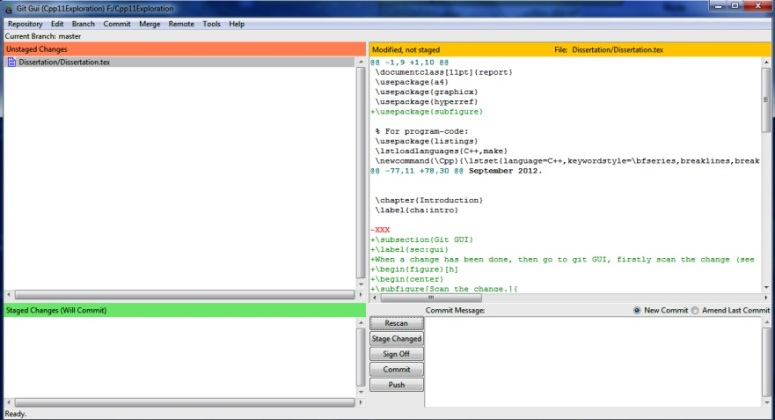
\includegraphics[scale=0.50]{../GitPhotos/GitScan.jpg}
\caption{Scan the modification.}
\label{fig:gitscan}
\end{center}
\end{figure}
\begin{figure}[h]
\begin{center}
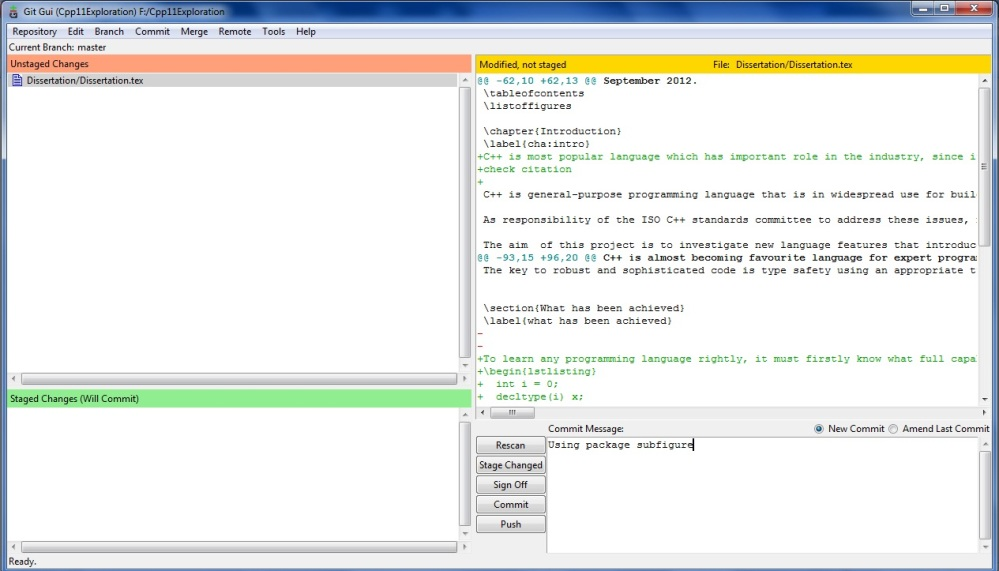
\includegraphics[scale=0.50]{../GitPhotos/GitCommand.jpg}
\caption{Write a command for the modification.}
\label{fig:gitcommand}
\end{center}
\end{figure}
\begin{figure}[h]
\begin{center}
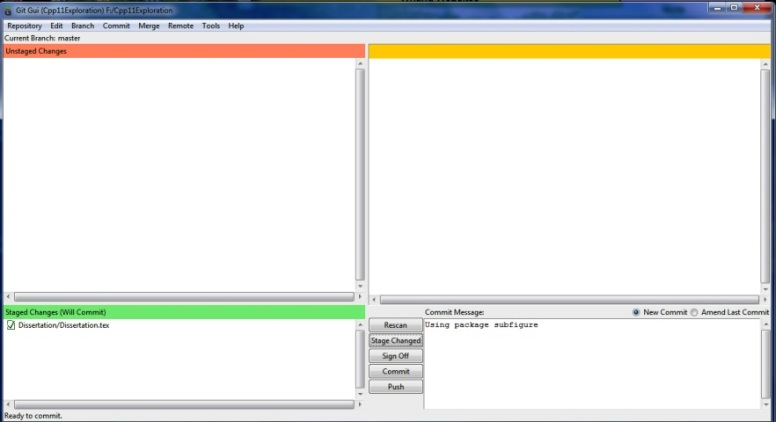
\includegraphics[scale=0.50]{../GitPhotos/GitStage.jpg}
\caption{Stage the modification.}
\label{fig:gitstage}
\end{center}
\end{figure}
\begin{figure}[h]
\begin{center}
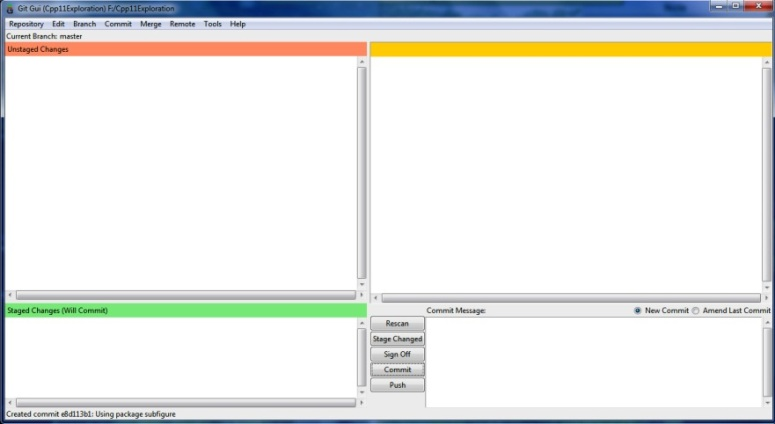
\includegraphics[scale=0.50]{../GitPhotos/GitCommit.jpg}
\caption{Commit the modification.}
\label{fig:gitcommit}
\end{center}
\end{figure}

\subsection{Why is Git used?}
\label{subsec: why git}
Developing such the large project requires a great tool for managing source code efficiently as well as allowed other contributors to work on project simultaneously to being developed faster. Git offers such mechanism that making contributions possible on repositories. Therefore, Git is used by Dr.~Kullmann and I to follow this project over period of allowed time. It was very helpful to me to get corrections, suggestions and guidance from Dr.~Kullmann about the right way to achieve this project successfully.

\section{Make utility}
\label{sec: Make}
The traditional mechanics of compiling the source file into an executable file that used by several programmers could be useful, when program is fairly simple. However, the situation is not when a program contains a lot of small pieces of programs and need to be compiled, because programmers face difficult to deal with modification of files when are done to fix the bug. Thus, handling many files need a great tool that offer facilities to create executable file in such easy way as well as compiling only modified files instead of all source files. Therefore, Make utility is used as solution for such situation.

The Make utility is "a tool automatically determines which pieces of a large program need to be recompiled, and issues commands to recompile them " (for further information see~\cite{Stallman:2000:GnuMake},~p.~5). Make is designed to allow programmers to efficiently compile large complex programs with many components easily. It provides mechanism to compile and turn source code into executable program with minimum effort. This is done by writing only "make" command in the UNIX shell. Make utility is especially helpful to manage and organizing projects that comprised of many source files and it reduces the probability of human error and difficulty of compilation.

\subsection{How does Make work?}
\label{subsec: how make work}
In UNIX, when "make" command is typed; the operating system looks at file called "makefile" which residents in the directory of where programs reside. Makefile contains a series of directives and knowledge that tell "make" how to compile source files and in what order. Make goes through a makefile commencing with the target which going to create and it also looks at dependencies of each target to find whether they are also considered as targets.  Make traces the chain of dependencies till it attains the end of the chain. At that time, it starts returning out to execute the commands that have been found in each target's rule (for addition information see~\cite{Stallman:2000:GnuMake},~p.~18). Building executable files by make, commences with building object files from the source files, and then links those objects files to create executable files. if any of source files is modified, the make utility compile only its object file and then linked into executable file, rather than recompiling all the source files. Therefore, running make utility is only possible if Makefile is provided within same directory and its contain all descriptions are required for directing make.

\subsection{Makefile}
\label{subsec: makefile}
Makefile is file that contains full directive of the commands (for more details see~\cite{Mecklenburg:2004:MakeGun},~p.~3) used by make to decide how to build and execute the programs. It specifies the relationships between the component and target files of project by listing the needed files for each target file. In general, Makefile contains at least two basic components macros and rules, and both are included in the Makefile that used in this project(see~\ref{Makefile}).

\begin{enumerate}
\item \textbf{Macro} Basically macro is a name or alias that is used to represent a string or instruction which could use frequently within the Makefile. It is considered a very helpful way to simplify contains of Makefile. Macro is defined in Makefile by a programmer through using (=) operator just like variables in C++ and convert it into its value in a target that is used for, require enclosing it within \$~( ). Furthermore, there are internal macros that predefined in make to do specific purpose. These internal macros are very helpful to avoid code duplication. Macros that used by programmer in Makefile for this project are:

\begin{enumerate}


\item \begin{verbatim}
CXX = g++ 
\end{verbatim}
Assign g++ compiler to macro called CXX to compile all C++ programs.


\item \begin{verbatim}
standard_options = -std=c++11 -Wall -pedantic
\end{verbatim}
Assign several options together such as (-Wall) that enable all warning during compiling process, and add the command-line parameter -std = c++11 to support C++11 features.

\item \begin{verbatim}
source_dir = .
\end{verbatim}
Assign directory, which used to find all files that have extension (such as cpp files)  to macro called source\_dir.

\item \begin{verbatim}
bin_dir = bin
\end{verbatim}
Assign directory called bin which contains all executable programs that produced by make, to macro called bin\_dir.

\item \begin{verbatim}
core_runtime = CoreLanguage/RunTime
core_functionality = CoreLanguage/FunctionalityImprovements
core_usability = CoreLanguage/UsabilityEnhancements
\end{verbatim}
Assign path of directories, to macros core\_runtime, core\_functionality and core\_usability which contain all programs of project.

\item \begin{verbatim}
compilation_units = $(wildcard $(source_dir)/*.cpp)
\end{verbatim}
Assign wildcard function that used to get a list of all cpp files from directories (core\_runtime, core\_functionality and core\_usability), to macro called compilation\_units.

\item \begin{verbatim}
source_files = $(notdir $(compilation_units))
\end{verbatim}
Assign notdir function that used to extract all files from (compilation\_units) which contains all files, to macro called source\_files.

\item \begin{verbatim}
programs = $(addprefix $(bin_dir)/, $(source_files:.cpp=))
\end{verbatim}
assign addprefix function that takes (source\_files:cpp) as a series of files and (bin\_dir) as directory to build lists of source files, to macro program.
\end{enumerate}

\item \textbf{Rules} Rule is very crucial in Make utility, since it tells Make when and how to remake files. In general, its syntax looks like follows:
\begin{verbatim}
target ... : Prerequisites....
<tap>        command ...
             command ...
\end{verbatim}

\begin{enumerate}
\item \textbf{Targets} Targets are the core of what a Makefile does. They represent the name of required files that must be generated by a program such as executable or object files. They can also represent the name of an action to accomplish such as "clean".

\item \textbf{Prerequisites} Prerequisites (also called dependence) are files that are used as input to generate the targets.

\item \textbf{Commands} Commands are action that will generate the targets from the prerequisites. The rule may contain more than command and each has its own line as showed above.
\end{enumerate}

Rules can be classified into explicit and implicit rules. 
\begin{enumerate}
\item \textbf{Explicit rules} Explicit rules are used to specify particular files as targets and prerequisites. In this type, a specific target will be updated whenever it is out of date, regarding to any of its prerequisites.

Explicit rules are used in our Makefile to do some purposes as follows:
\begin{enumerate}
\item \begin{verbatim}
.PHONY : all cleanall
\end{verbatim}
A phony is explicit target that used to avoid a conflict with a file of the same name, and to improve performance. Phony target is not really the name of file but it just use as recipe to be executed when there is an explicit request. By using phony target in this Makefile, make will run (all cleanall) regardless of whether there are files named (all cleanall).

\item \begin{verbatim}
cleanall :
\end{verbatim}
Cleanall is explicit target that used to delete all the object files and executable files but here it defined in the beginning as phony target.
\end{enumerate}

\item \textbf{Implicit rules} Implicit rules are general rule that tell make utility when and how to build files that has specific file extensions. Implicit rules begin with either a period or path and can be either suffix rules or pattern rules. Suffix rules are built into make and used as default rules to deal with C language.  Pattern rules are defined by using \% character and are used for matching common targets and prerequisites and built into make as well.

Implicit rules are used in our Makefile to achieve specific purpose:
\begin{enumerate}
\item \begin{verbatim}
.SUFFIXES :
\end{verbatim}
This used to delete all defaults suffix rules, and allowing us to define new rules that deal with C++ language.

\item \begin{verbatim}
$(programs) : $(bin_dir)/% : %.cpp
\end{verbatim}
Pattern rules are used for match specific files. Thus, we build our pattern rules which take any cpp file (\% .cpp) and put it in bin\_dir, and assign them to \$(programs), to be compiled.

\end{enumerate}
\end{enumerate}
\end{enumerate}


% conclsion
\chapter{Conclusion}
\label{chapter: conclusion}

\section{Summary}
\label{se : summary}
This project has investigated the features that introduced to core language by C++11, which offers much more than (old) C++. C++11 provide new style of programming that able to avoid inherently vulnerable facilities. It also offers significant features that improve the performance of programs in real-time.

C++11 simplify the syntax of language and make it more usable and much easier to understand. This has positive influence to bring newcomers programmers from both traditional C++ and other languages. Furthermore, it brings new facilities that able to do something extraordinary with little effort.  C++11 furnish new features that existed in most modern language and allows programmers to achieve what they expected to achieve with other languages.

However, C++11 is not able to cover all limitations of traditional C++, but will not bring new loopholes that making programming unsafe.

\section{Future work}
\label{sec: future work}
Development of this project was only restricted on investigation of core language which has been classified according to features that belong to. This project can be extended to become holistic by investigating features that added to libraries such as Standard Library (including thread library), and STL container, STL algorithms and Boost library, and present them as reference library to support programmers who have knowledge in C++ and want to program in C++11 style. Doing that, will give programmers an idea of the aims of the ISO C++ standards effort and actual capability of C++11 in real-time.

\section{Personal experience}
\label{sec: personal experience}
Developing this project successfully overcame three major challenges.  Each of which raised some difficulties during investigation of this project. The first challenge was finding resource related to this project, due to that fact that the project was commencing in the early  2012 and new standard C++11 was released in late  2011. The second challenge was dealing with unfamiliar functionality and syntax that existed in some features such as variadic template and lambda expression. Because of my experience is only restricted in C++, nor do other modern languages and seeing such things extraordinary require thinking in depth. The final challenge was demonstrating all cases of each feature in simple way to become understandable for programmer from first glance, this require to make program neglects some aspect and focus on the others.

Overall this project has given me unique chance to learn new style of programming with new language that could change the world. It has also provided me the opportunity to practice my knowledge in C++ and discover strength and weakness of it. Furthermore, I learnt Git and Make tools that make me able to manage and evolve large projects in the near future. My greatest achievement during developing this project was knowing the possibility of each feature and when should be applied to write elegant and efficient code. This makes me able to build some application that fit my purposes. I have learnt many worthwhile skills from this project which will have significant influence over my future.

% References
\addcontentsline{toc}{section}{Bibliography}
\bibliographystyle{alpha}
\bibliography{Bibliography}	


\begin{appendix}

\chapter{Program Code}
\label{chapter:Programcode}


\section{MakeFile}
\label{Makefile}

\Make

\lstinputlisting{../Makefile.}


% Core language Runtime Performance Enhancements
\section{Core Language Runtime Performance Enhancements}
\label{Appendix: corelanguage runtime performance}

\Cpp

% Rvalue reference
\subsection{RvalueReference\_Basic.cpp}
\label{RvalueReference_Basic}
\lstinputlisting{../CoreLanguage/RunTime/RvalueReference_Basic.cpp}

\subsection{RvalueReference\_Parameter.cpp}
\label{RvalueReference_Parameter}
\lstinputlisting{../CoreLanguage/RunTime/RvalueReference_Parameter.cpp}

\subsection{RvalueReference\_Move.cpp}
\label{RvalueReference_Move}
\lstinputlisting{../CoreLanguage/RunTime/RvalueReference_Move.cpp}

\subsection{RvalueReference\_Template.cpp}
\label{RvalueReference_Template}
\lstinputlisting{../CoreLanguage/RunTime/RvalueReference_Template.cpp}

\subsection{RvalueReference\_Forwarding.cpp}
\label{RvalueReference_Forwarding}
\lstinputlisting{../CoreLanguage/RunTime/RvalueReference_Forwarding.cpp}

% Move semantic
\subsection{MoveSemantic\_Constructor.cpp}
\label{MoveSemantic_Constructor}
\lstinputlisting{../CoreLanguage/RunTime/MoveSemantic_Constructor.cpp}

\subsection{MoveSemantic\_AssignmentOperator.cpp}
\label{MoveSemantic_AssignmentOperator}
\lstinputlisting{../CoreLanguage/RunTime/MoveSemantic_AssignmentOperator.cpp}

\subsection{MoveSemantic\_Swap.cpp}
\label{MoveSemantic_Swap}
\lstinputlisting{../CoreLanguage/RunTime/MoveSemantic_Swap.cpp}

% Generliazed constant expression
\subsection{Constexpr\_Data.cpp}
\label{Constexpr_Data}
\lstinputlisting{../CoreLanguage/RunTime/Constexpr_Data.cpp}

\subsection{Constexpr\_Recursion.cpp}
\label{Constexpr_Recursion}
\lstinputlisting{../CoreLanguage/RunTime/Constexpr_Recursion.cpp}

\subsection{Constexpr\_ArraySize.cpp}
\label{Constexpr_ArraySize}
\lstinputlisting{../CoreLanguage/RunTime/Constexpr_ArraySize.cpp}

\subsection{Constexpr\_FunctionRuntime.cpp}
\label{Constexpr_FunctionRuntime}
\lstinputlisting{../CoreLanguage/RunTime/Constexpr_FunctionRuntime.cpp}

\subsection{Constexpr\_ConstantConstructor.cpp}
\label{Constexpr_ConstantConstructor}
\lstinputlisting{../CoreLanguage/RunTime/Constexpr_ConstantConstructor.cpp}

% POD
\subsection{POD\_TrivialClass.cpp}
\label{POD_TrivialClass}
\lstinputlisting{../CoreLanguage/RunTime/POD_TrivialClass.cpp}

\subsection{POD\_StandardLayoutClass.cpp}
\label{POD_StandardLayoutClass}
\lstinputlisting{../CoreLanguage/RunTime/POD_StandardLayoutClass.cpp}

\subsection{POD\_StandardLayoutandTrivialClass.cpp}
\label{POD_StandardLayoutandTrivialClass}
\lstinputlisting{../CoreLanguage/RunTime/POD_StandardLayoutandTrivialClass.cpp}

% Core Language Usability Enhancements
\section{Core Language Usability Enhancements}
\label{Appendix: corelanguage usabiliy enhancements}

\Cpp

% Uniform initialization
\subsection{UniformInitialization\_ClassMembers.cpp}
\label{UniformInitialization_ClassMembers}
\lstinputlisting{../CoreLanguage/UsabilityEnhancements/UniformInitialization_ClassMembers.cpp}

\subsection{UniformInitialization\_Array.cpp}
\label{UniformInitialization_Array}
\lstinputlisting{../CoreLanguage/UsabilityEnhancements/UniformInitialization_Array.cpp}

\subsection{UniformInitialization\_DynamicArray.cpp}
\label{UniformInitialization_DynamicArray}
\lstinputlisting{../CoreLanguage/UsabilityEnhancements/UniformInitialization_DynamicArray.cpp}

\subsection{UniformInitialization\_ObjectReturn.cpp}
\label{UniformInitialization_ObjectReturn}
\lstinputlisting{../CoreLanguage/UsabilityEnhancements/UniformInitialization_ObjectReturn.cpp}

\subsection{UniformInitialization\_Narrowing.cpp}
\label{UniformInitialization_Narrowing}
\lstinputlisting{../CoreLanguage/UsabilityEnhancements/UniformInitialization_Narrowing.cpp}

% Initializer list
\subsection{InitializerList\_Constructor.cpp}
\label{InitializerList_Constructor}
\lstinputlisting{../CoreLanguage/UsabilityEnhancements/InitializerList_Constructor.cpp}

\subsection{InitializerList\_Vector.cpp}
\label{InitializerList_Vector}
\lstinputlisting{../CoreLanguage/UsabilityEnhancements/InitializerList_Vector.cpp}

\subsection{InitializerList\_Function.cpp}
\label{InitializerList_Function}
\lstinputlisting{../CoreLanguage/UsabilityEnhancements/InitializerList_Function.cpp}

% Auto keyword
\subsection{AutoKeyword\_Variable.cpp}
\label{AutoKeyword_Variable}
\lstinputlisting{../CoreLanguage/UsabilityEnhancements/AutoKeyword_Variable.cpp}

\subsection{AutoKeyword\_ConstVolatile.cpp}
\label{AutoKeyword_ConstVolatile}
\lstinputlisting{../CoreLanguage/UsabilityEnhancements/AutoKeyword_ConstVolatile.cpp}

\subsection{AutoKeyword\_NewExpression.cpp}
\label{AutoKeyword_NewExpression}
\lstinputlisting{../CoreLanguage/UsabilityEnhancements/AutoKeyword_NewExpression.cpp}

\subsection{AutoKeyword\_Function.cpp}
\label{AutoKeyword_Function}
\lstinputlisting{../CoreLanguage/UsabilityEnhancements/AutoKeyword_Function.cpp}

\subsection{AutoKeyword\_MapContainer.cpp}
\label{AutoKeyword_MapContainer}
\lstinputlisting{../CoreLanguage/UsabilityEnhancements/AutoKeyword_MapContainer.cpp}

\subsection{AutoKeyword\_InitializerList.cpp}
\label{AutoKeyword_InitializerList}
\lstinputlisting{../CoreLanguage/UsabilityEnhancements/AutoKeyword_InitializerList.cpp}

\subsection{AutoKeyword\_Template.cpp}
\label{AutoKeyword_Template}
\lstinputlisting{../CoreLanguage/UsabilityEnhancements/AutoKeyword_Template.cpp}

% Decltype keyword
\subsection{DecltypeKeyword\_Variable.cpp}
\label{DecltypeKeyword_Variable}
\lstinputlisting{../CoreLanguage/UsabilityEnhancements/DecltypeKeyword_Variable.cpp}

\subsection{DecltypeKeyword\_lvalue.cpp}
\label{DecltypeKeyword_lvalue}
\lstinputlisting{../CoreLanguage/UsabilityEnhancements/DecltypeKeyword_lvalue.cpp}

\subsection{DecltypeKeyword\_Function.cpp}
\label{DecltypeKeyword_Function}
\lstinputlisting{../CoreLanguage/UsabilityEnhancements/DecltypeKeyword_Function.cpp}

\subsection{DecltypeKeyword\_Template.cpp}
\label{DecltypeKeyword_Template}
\lstinputlisting{../CoreLanguage/UsabilityEnhancements/DecltypeKeyword_Template.cpp}

% alternative function syntax
\subsection{AlternativeFunction\_Syntax.cpp}
\label{AlternativeFunction_Syntax}
\lstinputlisting{../CoreLanguage/UsabilityEnhancements/AlternativeFunction_Syntax.cpp}

\subsection{AlternativeFunction\_This.cpp}
\label{AlternativeFunction_This}
\lstinputlisting{../CoreLanguage/UsabilityEnhancements/AlternativeFunction_This.cpp}

\subsection{AlternativeFunction\_Template.cpp}
\label{AlternativeFunction_Template}
\lstinputlisting{../CoreLanguage/UsabilityEnhancements/AlternativeFunction_Template.cpp}

\subsection{AlternativeFunction\_Scope.cpp}
\label{AlternativeFunction_Scope}
\lstinputlisting{../CoreLanguage/UsabilityEnhancements/AlternativeFunction_Scope.cpp}

% Ragne-based for statement
\subsection{RangeFor\_Array.cpp}
\label{RangeFor_Array}
\lstinputlisting{../CoreLanguage/UsabilityEnhancements/RangeFor_Array.cpp}

\subsection{RangeFor\_InitializerList.cpp}
\label{RangeFor_InitializerList}
\lstinputlisting{../CoreLanguage/UsabilityEnhancements/RangeFor_InitializerList.cpp}

\subsection{RangeFor\_Vector.cpp}
\label{RangeFor_Vector}
\lstinputlisting{../CoreLanguage/UsabilityEnhancements/RangeFor_Vector.cpp}

\subsection{RangeFor\_UniformInitialization.cpp}
\label{RangeFor_UniformInitialization}
\lstinputlisting{../CoreLanguage/UsabilityEnhancements/RangeFor_UniformInitialization.cpp}

% Lambda Expression
\subsection{Lambda\_Mutable.cpp}
\label{Lambda_Mutable}
\lstinputlisting{../CoreLanguage/UsabilityEnhancements/Lambda_Mutable.cpp}

\subsection{Lambda\_FunctionParameter.cpp}
\label{Lambda_FunctionParameter}
\lstinputlisting{../CoreLanguage/UsabilityEnhancements/Lambda_FunctionParameter.cpp}

\subsection{Lambda\_Invocation.cpp}
\label{Lambda_Invocation}
\lstinputlisting{../CoreLanguage/UsabilityEnhancements/Lambda_Invocation.cpp}

\subsection{Lambda\_Foreach.cpp}
\label{Lambda_Foreach}
\lstinputlisting{../CoreLanguage/UsabilityEnhancements/Lambda_Foreach.cpp}

\subsection{Lambda\_ExplicitReturn.cpp}
\label{Lambda_ExplicitReturn}
\lstinputlisting{../CoreLanguage/UsabilityEnhancements/Lambda_ExplicitReturn.cpp}

\subsection{Lambda\_ImplicitReturn.cpp}
\label{Lambda_ImplicitReturn}
\lstinputlisting{../CoreLanguage/UsabilityEnhancements/Lambda_ImplicitReturn.cpp}

\subsection{Lambda\_PointerFunction.cpp}
\label{Lambda_PointerFunction}
\lstinputlisting{../CoreLanguage/UsabilityEnhancements/Lambda_PointerFunction.cpp}

\subsection{Lambda\_FunctionReturnType.cpp}
\label{Lambda_FunctionReturnType}
\lstinputlisting{../CoreLanguage/UsabilityEnhancements/Lambda_FunctionReturnType.cpp}

\subsection{Lambda\_Sort.cpp}
\label{Lambda_Sort}
\lstinputlisting{../CoreLanguage/UsabilityEnhancements/Lambda_Sort.cpp}

% Delegating Constructors
\subsection{DelegatingConstructor.cpp}
\label{DelegatingConstructor}
\lstinputlisting{../CoreLanguage/UsabilityEnhancements/DelegatingConstructor.cpp}

% Override keyword
\subsection{OverrideKeyword.cpp}
\label{OverrideKeyword}
\lstinputlisting{../CoreLanguage/UsabilityEnhancements/OverrideKeyword.cpp}

% Final keyword
\subsection{FinalKeyword.cpp}
\label{FinalKeyword}
\lstinputlisting{../CoreLanguage/UsabilityEnhancements/FinalKeyword.cpp}

% Null pointer constant
\subsection{NullPointer.cpp}
\label{NullPointer}
\lstinputlisting{../CoreLanguage/UsabilityEnhancements/NullPointer.cpp}

% Strongly Typed Enumerations
\subsection{EnumerationClass\_Implicit.cpp}
\label{EnumerationClass_Implicit}
\lstinputlisting{../CoreLanguage/UsabilityEnhancements/EnumerationClass_Implicit.cpp}

\subsection{EnumerationClass\_Explicit.cpp}
\label{EnumerationClass_Explicit}
\lstinputlisting{../CoreLanguage/UsabilityEnhancements/EnumerationClass_Explicit.cpp}

\subsection{EnumerationClass\_Conflict.cpp}
\label{EnumerationClass_Conflict}
\lstinputlisting{../CoreLanguage/UsabilityEnhancements/EnumerationClass_Conflict.cpp}

% Explicit conversion
\subsection{Explicit\_Constructor.cpp}
\label{Explicit_Constructor}
\lstinputlisting{../CoreLanguage/UsabilityEnhancements/Explicit_Constructor.cpp}

\subsection{Explicit\_Operator.cpp}
\label{Explicit_Operator}
\lstinputlisting{../CoreLanguage/UsabilityEnhancements/Explicit_Operator.cpp}

% Alias Template
\subsection{TypeAlias\_FunctionPointer.cpp}
\label{TypeAlias_FunctionPointer}
\lstinputlisting{../CoreLanguage/UsabilityEnhancements/TypeAlias_FunctionPointer.cpp}

\subsection{TypeAlias\_Varialbe.cpp}
\label{TypeAlias_Varialbe}
\lstinputlisting{../CoreLanguage/UsabilityEnhancements/TypeAlias_Variable.cpp}

\subsection{TypeAlias\_Template.cpp}
\label{TypeAlias_Template}
\lstinputlisting{../CoreLanguage/UsabilityEnhancements/TypeAlias_Template.cpp}



% Core Language Functionality Improvements
\section{Core Language Functionality Improvements}
\label{Appendix: corelanguage functionality improvements}

\Cpp

% NewCharacterType - char16 and char32
\subsection{NewCharacterType\_char16.cpp}
\label{NewCharacterType_char16}
\lstinputlisting{../CoreLanguage/FunctionalityImprovements/NewCharacterType_char16.cpp}

\subsection{NewCharacterType\_String16.cpp}
\label{NewCharacterType_String16}
\lstinputlisting{../CoreLanguage/FunctionalityImprovements/NewCharacterType_String16.cpp}

\subsection{NewCharacterType\_char32.cpp}
\label{NewCharacterType_char32}
\lstinputlisting{../CoreLanguage/FunctionalityImprovements/NewCharacterType_char32.cpp}

\subsection{NewCharacterType\_String32.cpp}
\label{NewCharacterType_String32}
\lstinputlisting{../CoreLanguage/FunctionalityImprovements/NewCharacterType_String32.cpp}

\subsection{NewCharacterType\_UTF-8.cpp}
\label{NewCharacterType_UTF-8}
\lstinputlisting{../CoreLanguage/FunctionalityImprovements/NewCharacterType_UTF-8.cpp}

\subsection{NewCharacterType\_Languages.cpp}
\label{NewCharacterType_Languages}
\lstinputlisting{../CoreLanguage/FunctionalityImprovements/NewCharacterType_Languages.cpp}

% Raw string literals
\subsection{RawString\_Backslash.cpp}
\label{RawString_Backslash}
\lstinputlisting{../CoreLanguage/FunctionalityImprovements/RawString_Backslash.cpp}

\subsection{RawString\_EscapeSequence.cpp}
\label{RawString_EscapeSequence}
\lstinputlisting{../CoreLanguage/FunctionalityImprovements/RawString_EscapeSequence.cpp}

\subsection{RawString\_HTML.cpp}
\label{RawString_HTML}
\lstinputlisting{../CoreLanguage/FunctionalityImprovements/RawString_HTML.cpp}

\subsection{RawString\_UnicodeliteralPrefix.cpp}
\label{RawString_UnicodeliteralPrefix}
\lstinputlisting{../CoreLanguage/FunctionalityImprovements/RawString_UnicodeliteralPrefix.cpp}

% User-defined literals
\subsection{UserLiterals\_LiteralOperators.cpp}
\label{UserLiterals_LiteralOperators}
\lstinputlisting{../CoreLanguage/FunctionalityImprovements/UserLiterals_LiteralOperators.cpp}

\subsection{UserLiterals\_RawStyle.cpp}
\label{UserLiterals_RawStyle}
\lstinputlisting{../CoreLanguage/FunctionalityImprovements/UserLiterals_RawStyle.cpp}

\subsection{UserLiterals\_CookedStyle1.cpp}
\label{UserLiterals_CookedStyle1}
\lstinputlisting{../CoreLanguage/FunctionalityImprovements/UserLiterals_CookedStyle1.cpp}

\subsection{UserLiterals\_CookedStyle2.cpp}
\label{UserLiterals_CookedStyle2}
\lstinputlisting{../CoreLanguage/FunctionalityImprovements/UserLiterals_CookedStyle2.cpp}

\subsection{UserLiterals\_CookedObject.cpp}
\label{UserLiterals_CookedObject}
\lstinputlisting{../CoreLanguage/FunctionalityImprovements/UserLiterals_CookedObject.cpp}

% default keyword
\subsection{DefaultKeyword\_Constructor.cpp}
\label{DefaultKeyword_Constructor}
\lstinputlisting{../CoreLanguage/FunctionalityImprovements/DefaultKeyword_Constructor.cpp}

\subsection{DefaultKeyword\_ClassAccessibility.cpp}
\label{DefaultKeyword_ClassAccessibility}
\lstinputlisting{../CoreLanguage/FunctionalityImprovements/DefaultKeyword_ClassAccessibility.cpp}

% delete keyword
\subsection{DeleteKeyword\_ClassMove.cpp}
\label{DeleteKeyword_ClassMove}
\lstinputlisting{../CoreLanguage/FunctionalityImprovements/DeleteKeyword_ClassMove.cpp}

\subsection{DeleteKeyword\_NewExpression.cpp}
\label{DeleteKeyword_NewExpression}
\lstinputlisting{../CoreLanguage/FunctionalityImprovements/DeleteKeyword_NewExpression.cpp}

\subsection{DeleteKeyword\_Overload.cpp}
\label{DeleteKeyword_Overload}
\lstinputlisting{../CoreLanguage/FunctionalityImprovements/DeleteKeyword_Overload.cpp}

% long long 
\subsection{Long.cpp}
\label{Long}
\lstinputlisting{../CoreLanguage/FunctionalityImprovements/Long.cpp}

% unsinged long long
\subsection{UnsignedLong.cpp}
\label{UnsignedLong}
\lstinputlisting{../CoreLanguage/FunctionalityImprovements/UnsignedLong.cpp}

% static assert
\subsection{StaticAssert\_Namespace.cpp}
\label{StaticAssert_Namespace}
\lstinputlisting{../CoreLanguage/FunctionalityImprovements/StaticAssert_Namespace.cpp}

\subsection{StaticAssert\_ClassTemplate.cpp}
\label{StaticAssert_ClassTemplate}
\lstinputlisting{../CoreLanguage/FunctionalityImprovements/StaticAssert_ClassTemplate.cpp}

\subsection{StaticAssert\_TypeTraitSame.cpp}
\label{StaticAssert_TypeTraitSame}
\lstinputlisting{../CoreLanguage/FunctionalityImprovements/StaticAssert_TypeTraitSame.cpp}

\subsection{StaticAssert\_TypeTraitFloat.cpp}
\label{StaticAssert_TypeTraitFloat}
\lstinputlisting{../CoreLanguage/FunctionalityImprovements/StaticAssert_TypeTraitFloat.cpp}

% varidaci template
\subsection{VariadicTemplate\_Function.cpp}
\label{VariadicTemplate_Function}
\lstinputlisting{../CoreLanguage/FunctionalityImprovements/VariadicTemplate_Function.cpp}

\subsection{VariadicTemplate\_Function1.cpp}
\label{VariadicTemplate_Function1}
\lstinputlisting{../CoreLanguage/FunctionalityImprovements/VariadicTemplate_Function1.cpp}

\subsection{VariadicTemplate\_Tuple.cpp}
\label{VariadicTemplate_Tuple}
\lstinputlisting{../CoreLanguage/FunctionalityImprovements/VariadicTemplate_Tuple.cpp}

\subsection{VariadicTemplate\_Class.cpp}
\label{VariadicTemplate_Class}
\lstinputlisting{../CoreLanguage/FunctionalityImprovements/VariadicTemplate_Class.cpp}


\end{appendix}

\end{document}
